\documentclass[11pt]{amsart}
\usepackage{amsmath,amsfonts,amssymb,amsthm,verbatim,multirow,url,subfig,footnote,graphicx,array,xr,booktabs,placeins,float}
\usepackage[usenames,dvipsnames]{color}
%  \usepackage[style=numeric,
%  doi=false,
%  isbn=false,
%  url=false]{biblatex}
\usepackage[utf8]{inputenc}
\usepackage[T1]{fontenc}


\theoremstyle{plain}
\newtheorem{lema}{Lemma}
\newtheorem{coro}{Corollary}
\newtheorem{teo}{Theorem}
\newtheorem{prop}{Proposition}
\theoremstyle{definition}
\newtheorem{ap}{Assumption}
\newtheorem{defin}{Definition}
\theoremstyle{remark}
\newtheorem*{rk}{Remark}
\newcommand{\nn}{\mathbf}
\newcommand{\nns}{\boldsymbol}
\newcommand{\Hcal}{\mathcal H}

\newcommand{\bl}[1]{\color{ForestGreen}\textbf{[Bo: #1]}\normalcolor}
\newcommand{\lb}[1]{\color{MidnightBlue}\textbf{[LB: #1]}\normalcolor}
\newcommand{\jeg}[1]{\color{ProcessBlue}\textbf{[JEG: #1]}\normalcolor}


%\addbibresource{biblioteca.bib}

\begin{document}
\title[Paleoclimate Reconstruction using INLA.]{Efficient Reconstructions of Common Era Climate via Integrated Nested Laplace Approximations.}

\author{Luis A. Barboza}
\address{Centro de Investigacion en Matematica Pura y Aplicada (CIMPA)-Escuela
  de Matematica, Universidad de Costa Rica\\
San Jos\'e, Costa Rica}
\email{luisalberto.barboza@ucr.ac.cr}


\author{Julien Emile-Geay}
\address{Department of Earth Sciences \\
  University of Southern California \\
  Los Angeles, California, USA.
}
\email{julieneg@usc.edu}


\author{Bo Li}
\address{Department of Statistics \\
  University of Illinois at Urbana-Champaign \\
  Champaign, Illinois, USA.
}
\email{libo@illinois.edu}

\author{Wan He}


\date{\today}
%\date{December 20, 2014}
\keywords{INLA,Paleoclimate Reconstruction,Hierarchical Bayesian Model}
\subjclass[2010]{}
\maketitle

\begin{abstract}
A Paleolimate Reconstruction on the Common Era (1-2000AD) was performed using a
Hierarchical Bayesian Model from three sources of data: proxy data from PAGES2k
project dataset, HadCRUT4 temperature data from the Climatic Research Unit
at the University of East Anglia and external forcing data from several sources.
Instead of using the MCMC approach to solve for the latent variable, we used the
INLA algorithm that shows a similar approximation than previous studies. The use
of external forcings was tested by replace them with a fixed number of
BSplines in the latent equation. Classical goodness-of-fit measures show that there is not a significant
difference between the predictive ability of both approaches. 
\end{abstract}

\section{Introduction.}
\label{sec:intro}

Paleoclimate reconstructions represent statistical simplifications of more
complex processes at the climatic level and they allow us to understand the past
behavior of temperatures over a specific area, and also the future trend of
observed temperatures. \lb{Julien: Can you help me to add more details about the
importance of paleoclimate reconstructions from the physical point of view?}

Many methods have been developed to reconstruct the past climate:
Expectation-Maximization algorithm (\cite{Schneider2001,mann2005testing},
\cite{mann2007robust}, \cite{rutherford2003climate}, \cite{bradley2005proxy},
\cite{steig2009}), principal component regression
(\cite{luterbacher2004european}, \cite{Wahl2012}), canonical
correlation analysis (\cite{smerdon2010pseudoproxy}), pairwise comparison
(\cite{Hanhijarvi2013}, \cite{Gergis2016}), data assimilation (\cite{Hakim2016}) among
others. We put special emphasis on the hierarchical Bayesian method, since it is
a method that from the point of view of paleoclimatic reconstruction has the
advantage of uniting different sources of uncertainty in a natural way, in
particular this method joins the variability of the temperature series as a
latent process as well as the variability of those climatic and biological
variables that serve as approximations of this process. Many studies have been
conducted under this type of Bayesian models: \cite{boli1}, \cite{tingley1},
\cite{tingley2}, \cite{tingley2013_Ext}, \cite{werner2012pseudoproxy},
\cite{Barboza2014} among others. Some of these studies have used space-state
schemes to linearly relate information that comes from biological and historial
proxies together with information from external climatic forcings, for example
greenhouse gases, volcanism and solar radiation. Two problems arise in this
type of models: proxy dataset reduction and the complexity of the model vs its execution time.

In this article we will work with a set of open-access data (PAGES2k dataset)
that provides a set of organized time-series of climate proxies with different
temporal resolution. This ensures that our calculations are completely
reproducible and that they can be updated regularly as the dataset changes over
time. In order to deal with the reduction of the proxy dataset, we compared five
popular dimension reduction techniques that allow us to compute reduced proxies
under different temporal horizons and we were able to compare them through their
predictive capacity during a validation period. We also considered the model
developed in \cite{Barboza2014}, and we explored to make it more complex by
including more information from the proxy dataset, as well as by extending the
reconstruction period by 1000 years. The participation of external forces in the
hierarchical Bayesian model was tested by comparing its ability to describe the
average behavior of temperature anomalies with respect to a linear combination
of BSplines. Of course, this adds more complexity to the hierarchical model and
it becomes more necessary to solve the slow behavior of the adjustment process
when we employ MCMC techniques. This second challenge was successfully solved by
approximating the adjustment with INLA (Integrated Nested Laplace
Approximation), with which we were able to adjust Bayesian models with much
greater complexity than \cite{Barboza2014} in a much shorter period of time. 

The article is organized as follows...

\section{Datasets.}
\label{sec:data}

\subsection{Proxy data.}
The PAGES2k global multiproxy database is a ``community-driven effort to
synthesize all publicly-archived, temperature-sensitive proxy records of the
past 2,000 years'' (see \cite{Kaufman2014}, \cite{PAGES2KConsortium2013} and \cite{PAGES2kConsortium2017}). The main objective of this database is
to create a free information conglomerate that integrates temperature proxies
with different level of resolution, in order to develop climatic
reconstructions.

The dataset is composed by a collection of borehole, coral, documentary, glacier
ice, lake and marine 
sediment, sclerosponge, speleothem and tree-ring data; collected through 688
data series around the world. Each of those proxies
has different time horizons and this creates difficulties in the aggregation of
information in simpler variables.  In order to select proxies with high
predictive power, we first chose those series with large correlation with respect to
their closest spatial temperature record using the HadCRUT4.2 dataset. More
details on this ``screening'' procedure can be found in \cite{Emile-Geay2015}. Finally we get 257 proxies
that pass the previous procedure (see the first panel of Figure \ref{fig:proxy} with the spatial
distribution of the final proxies).   
\begin{figure}
  \centering
  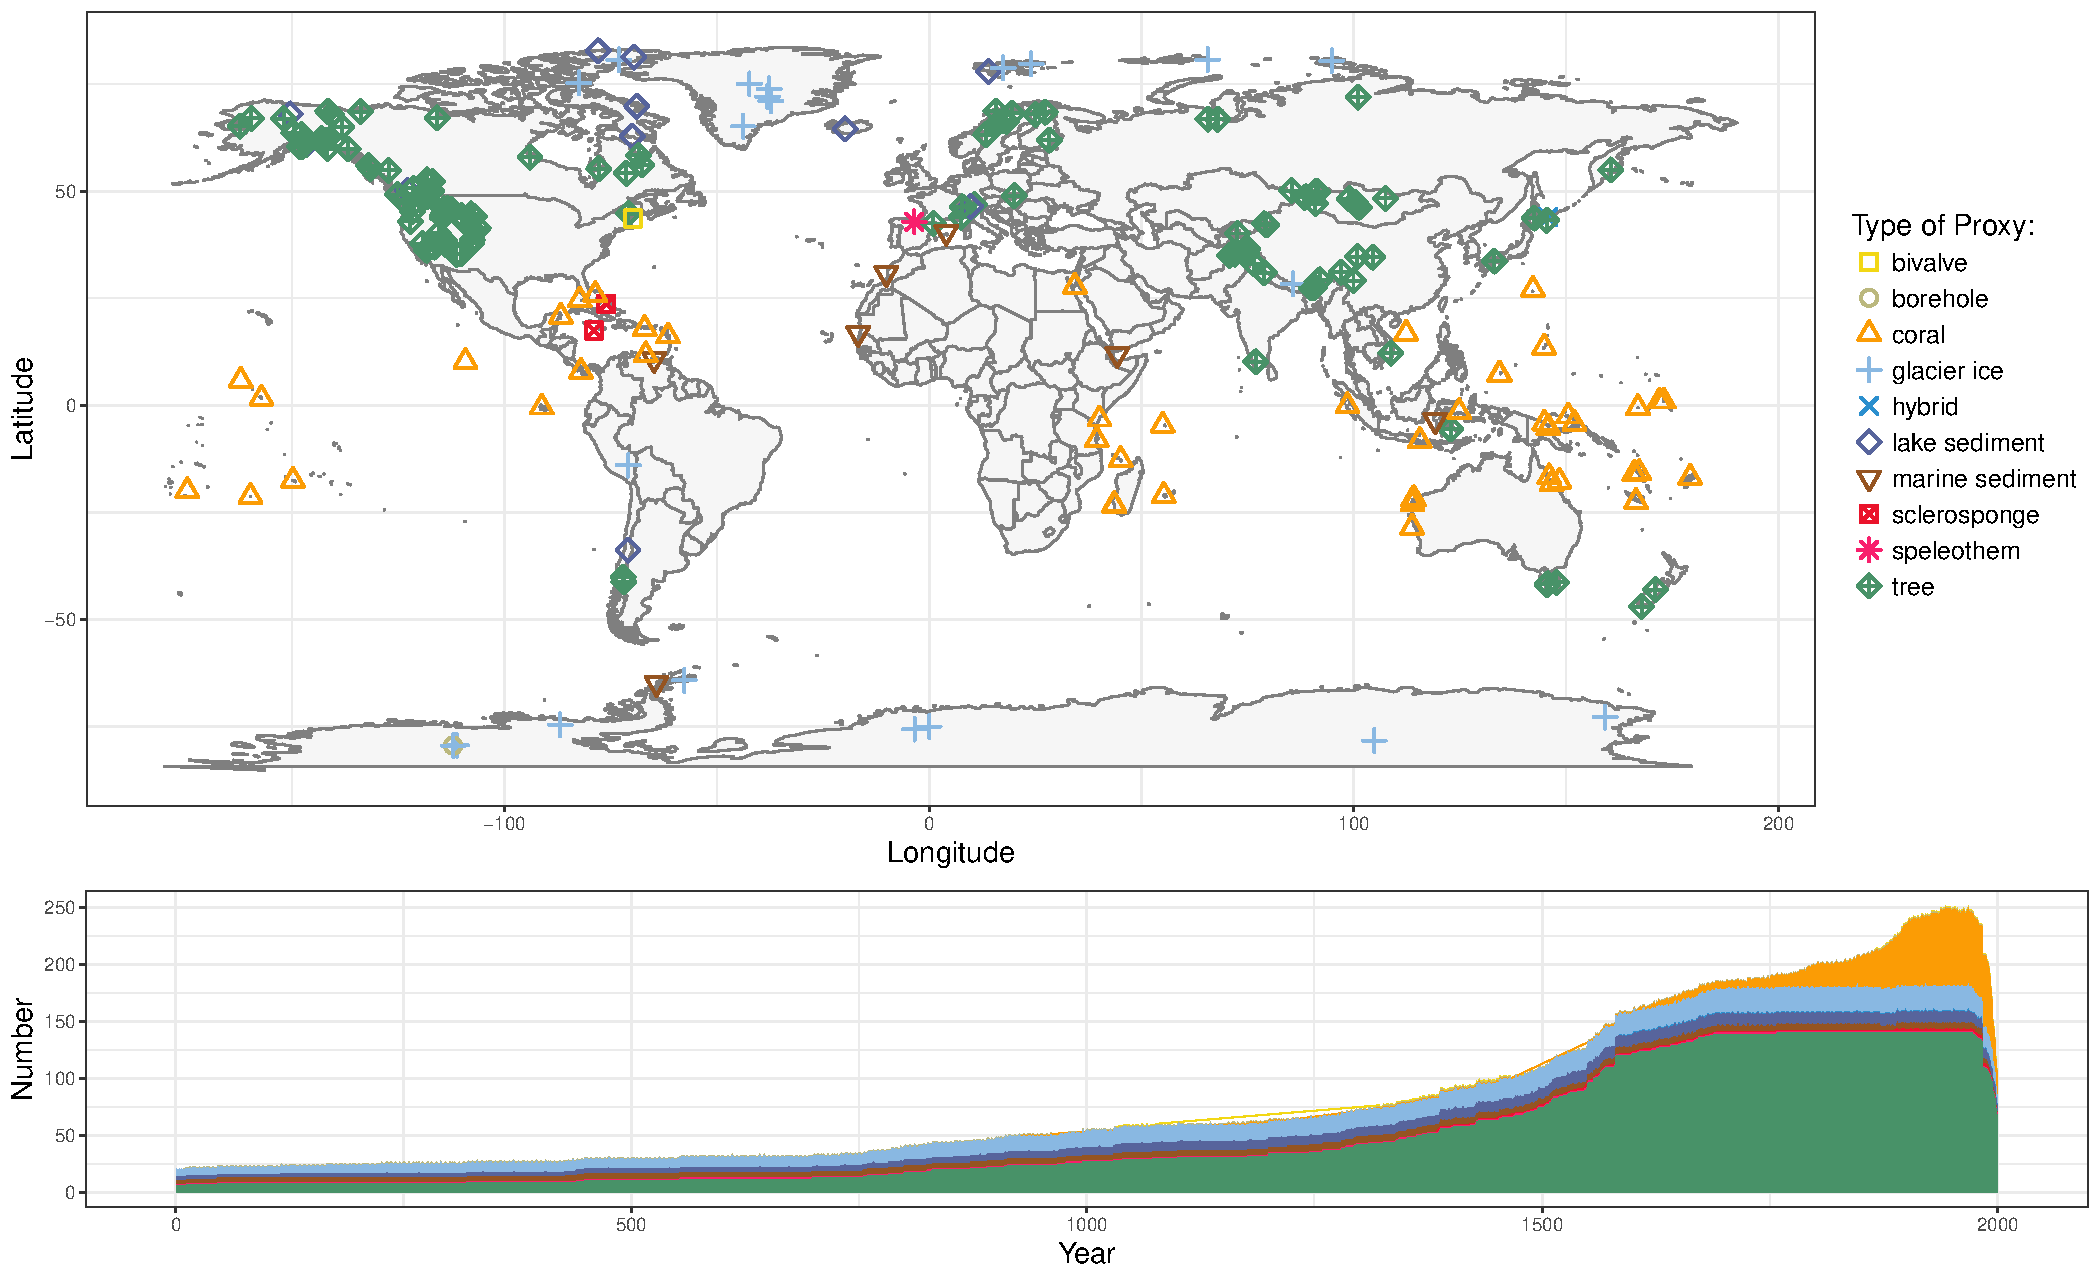
\includegraphics[scale=0.45]{CombinedMap_Area}
  \caption{Pages2k proxy distribution and temporal availability of proxies by
    type, after the screening procedure of \cite{Emile-Geay2015}.}
  \label{fig:proxy}
\end{figure}
As mentioned, proxies have different temporal horizons, as it can be shown in the
second panel of Figure~\ref{fig:proxy}. Unlike previous studies (for example \cite{Barboza2014}), in this article we try to take into account the information available in most proxies, despite their temporal diversity.


\subsection{Temperature data.}
We used the HadCRUT4 global temperature dataset provided by the Met Office Hadley
Centre and the Climatic Research Unit at the University of East Anglia, UK
(version 4.4.0.0). The dataset consists of instrumental, {\it in situ}
observations of surface temperature over land \cite{Jones2012} and ocean
\cite{Kennedy2011, Kennedy2011a}. The
observations are expressed as anomalies relative to the monthly-mean seasonal cycle over the 1961-1990 period in degrees Celsius. Though HadCRUT4 features a rather sophisticated analysis of error sources \cite{Morice2012}, including a 100-member ensemble of draws from the error distribution, we neglect these uncertainties against the much larger uncertainties affecting paleoclimate observations, and simply use the median of this ensemble, averaged on an annual basis.
\jeg{Note: it's a little too late for that, but one day it would be nice to
  incorporate the uncertainty in instrumental temperatures into your analysis.
  Perhaps mention this in the discussion as a possible application of
  INLA?}\lb{Yes, I will include that in the discussion.}

\subsection{Forcing data.}
The forcing data consists of (see Figure \ref{fig:forcings} in the Appendix):
\begin{itemize}
\item Historical Greenhouse-Gases concentrations: hemispheric means of mole
  fraction of carbon dioxide in air (ppm) with annual
  resolution, taken from Coupled Model Intercomparison Project (CMIP6) (see
  \cite{Meinshausen2016}).
  
\item Volcanic forcing from Easy Volcanic Aerosol (EVA) dataset (evolv2k): (see
  \cite{Toohey2016}) reconstructed zonal mean AOD (mid-visible, i.e., 550 nm), covering the
  500 BCE to 1900 CE time period. For 1900 (or 1850) to present, \cite{Thomason2016} is
  used to fill in the forcing table, the volcanic data at varying locations is
  weighted by cosine of their corresponding latitudes.
  
\item The solar forcing data is computed from SATIRE-H
  (Holocene) at \cite{Vieira2011}. Irradiance from SATIRE-H (Holocene) is
  recorded on a decadal basis from 9495BC - 1939AD and then on a daily basis
  from 1940AD onwards. Hence, the data prior to 1939AD was interpolated using splines and after 1940AD, an annual mean is computed. For consistence of resolution of the data, annual data from 1640AD to 2000AD is also spline interpolated.
\end{itemize}
All forcings are displayed in Figure~\ref{fig:forcings}.

\lb{Julien: Can you please include more details on this section?}

\begin{figure}
  \centering
  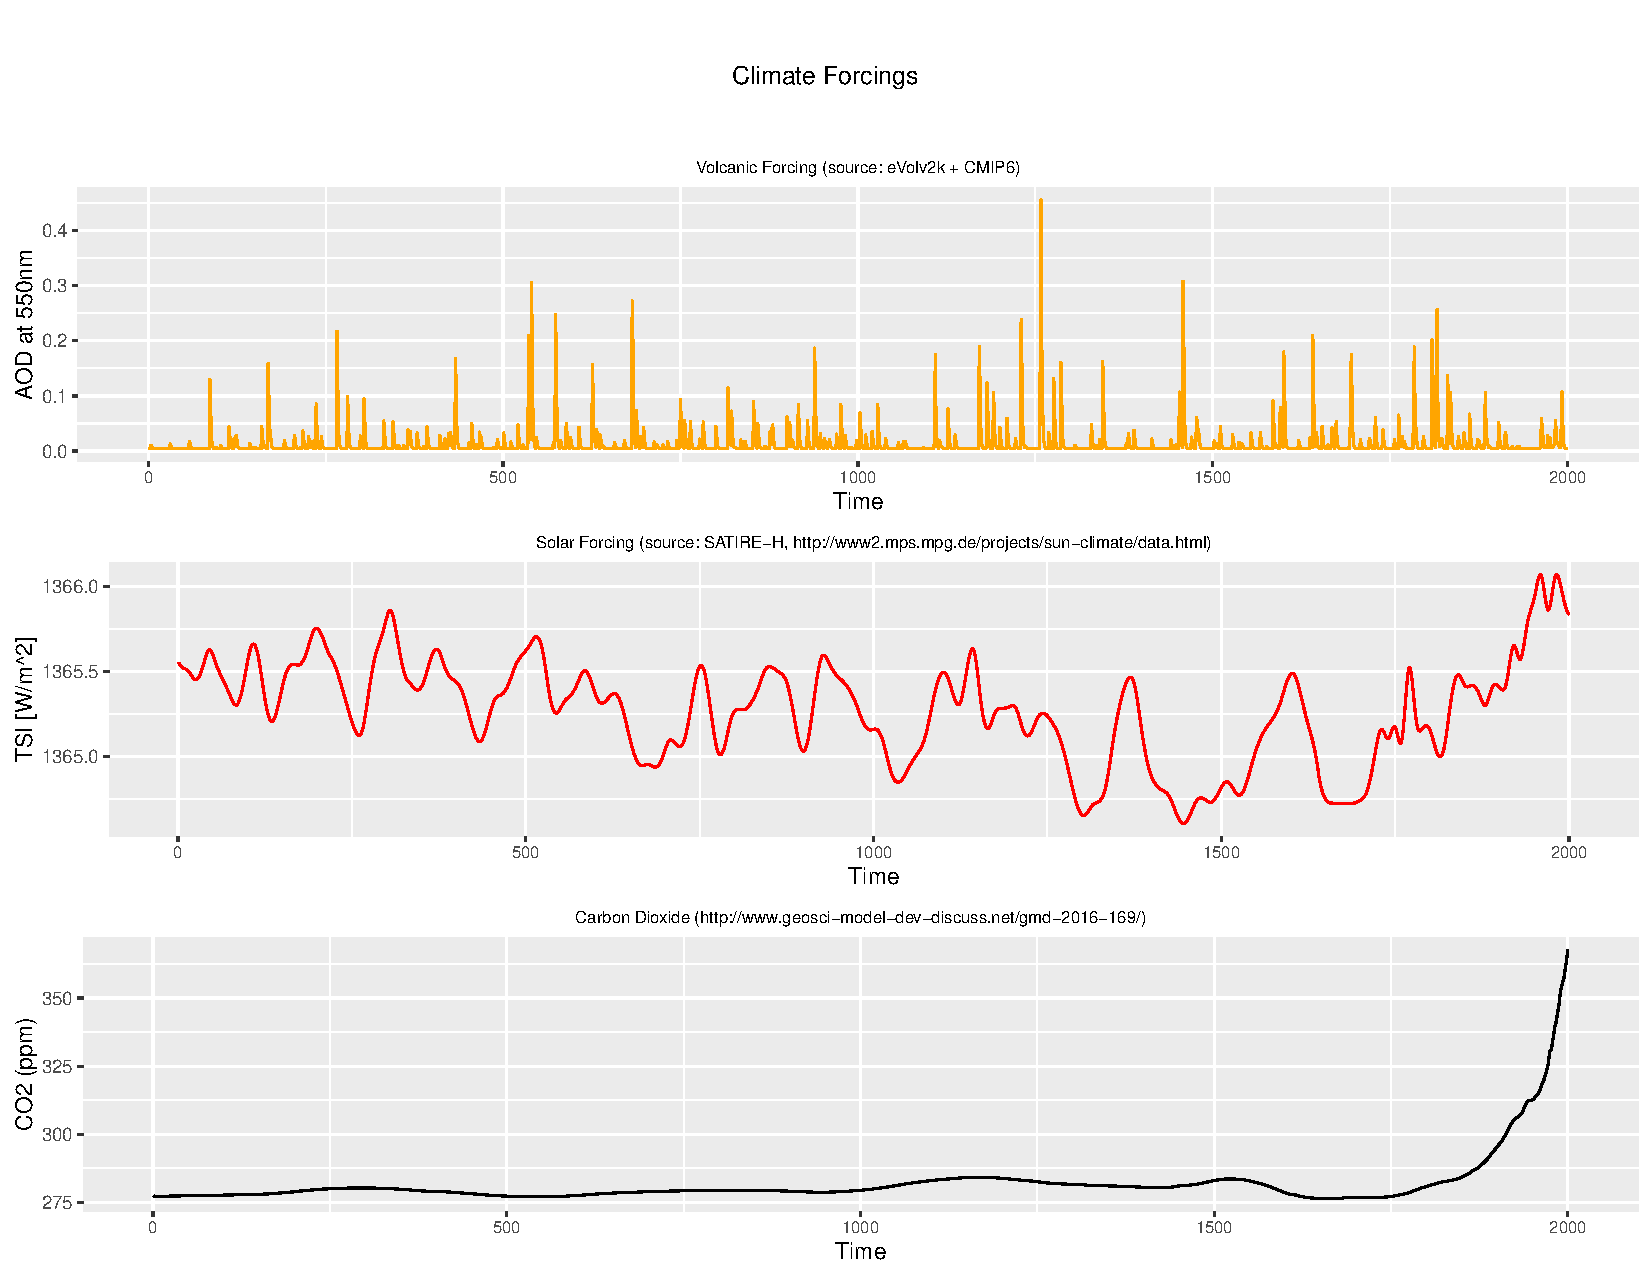
\includegraphics[scale=0.35]{forcings}
  \caption{Main climate Forcings of the Common Era (1-2000 AD): volcanic, solar, and carbon dioxide. AOD = Aerosol optical depth. TSI = total solar irradiance. ppm = parts per million. See text for details.}
  \label{fig:forcings}
\end{figure}

\section{Data reduction, modeling and computation}\label{sec:model}
\subsection{Data reduction methods}
\label{sec:rp}

The proxy data is massive due to the large number of proxies and their in-homogeneous temporal resolution and availability. The calibration period is however short compared to the number of proxies, therefore a typical large $p$ and small $n$ issue arises in the reconstruction. A data reduction is necessary and helpful in such situation. We will explore a few common data reduction methods.    

Following \cite{Barboza2014}, we reduce the dimension of the proxy dataset by
generating Reduced Proxy ($RP$) timeseries, which condense individual proxy
timeseries into a single timeseries with larger predictive power over the GMST
target.  The 257 proxy variables are first centered and scaled. Then we remove
proxy series whose proportion of missing annual observations is larger than 5\%
during the calibration  period.  \jeg{This gives me pause. Did you exclude all
  series lacking >5\% of data in a given 250y nest, or overall. If overall, you
  are missing out on a LOT of proxies!!! We should redo the calculations with a
  less restrictive threshold}\lb{The percentage of missing observations is
  computed over the calibration period (1900-2000), so we don't loose too much information.}. 

Due to the diversity of start dates in the proxies database (Fig. ~\ref{fig:proxy}), we gather proxies into non-homogeneous groups where each group has temporal availability within an
interval of 250 years. As the reconstruction is taking place over a 2000 year
horizon, this creates 8 groups with the distribution shown in Table \ref{tab:distdate}. The corresponding timeseries are displayed in Figure~\ref{fig:RPs}.
\begin{table}
  \centering
  \begin{tabular}{c|c|c}
    \toprule
    Group & Interval (year AD) & Number of Proxies\\
    \midrule
    1 & 1-250 & 19 \\
    2 & 251-500 & 25 \\
    3 & 501-750 & 29 \\
    4 & 751-1000 & 33 \\
    5 & 1001-1250 & 54 \\
    6 & 1251-1500 & 65 \\
    7 & 1501-1750 & 105 \\
    8 & 1751-2000 & 146 \\
    \bottomrule
  \end{tabular}
  \caption{Distribution of proxies according to their temporal availability.}
  \label{tab:distdate}
\end{table}

\begin{figure}
  \centering
 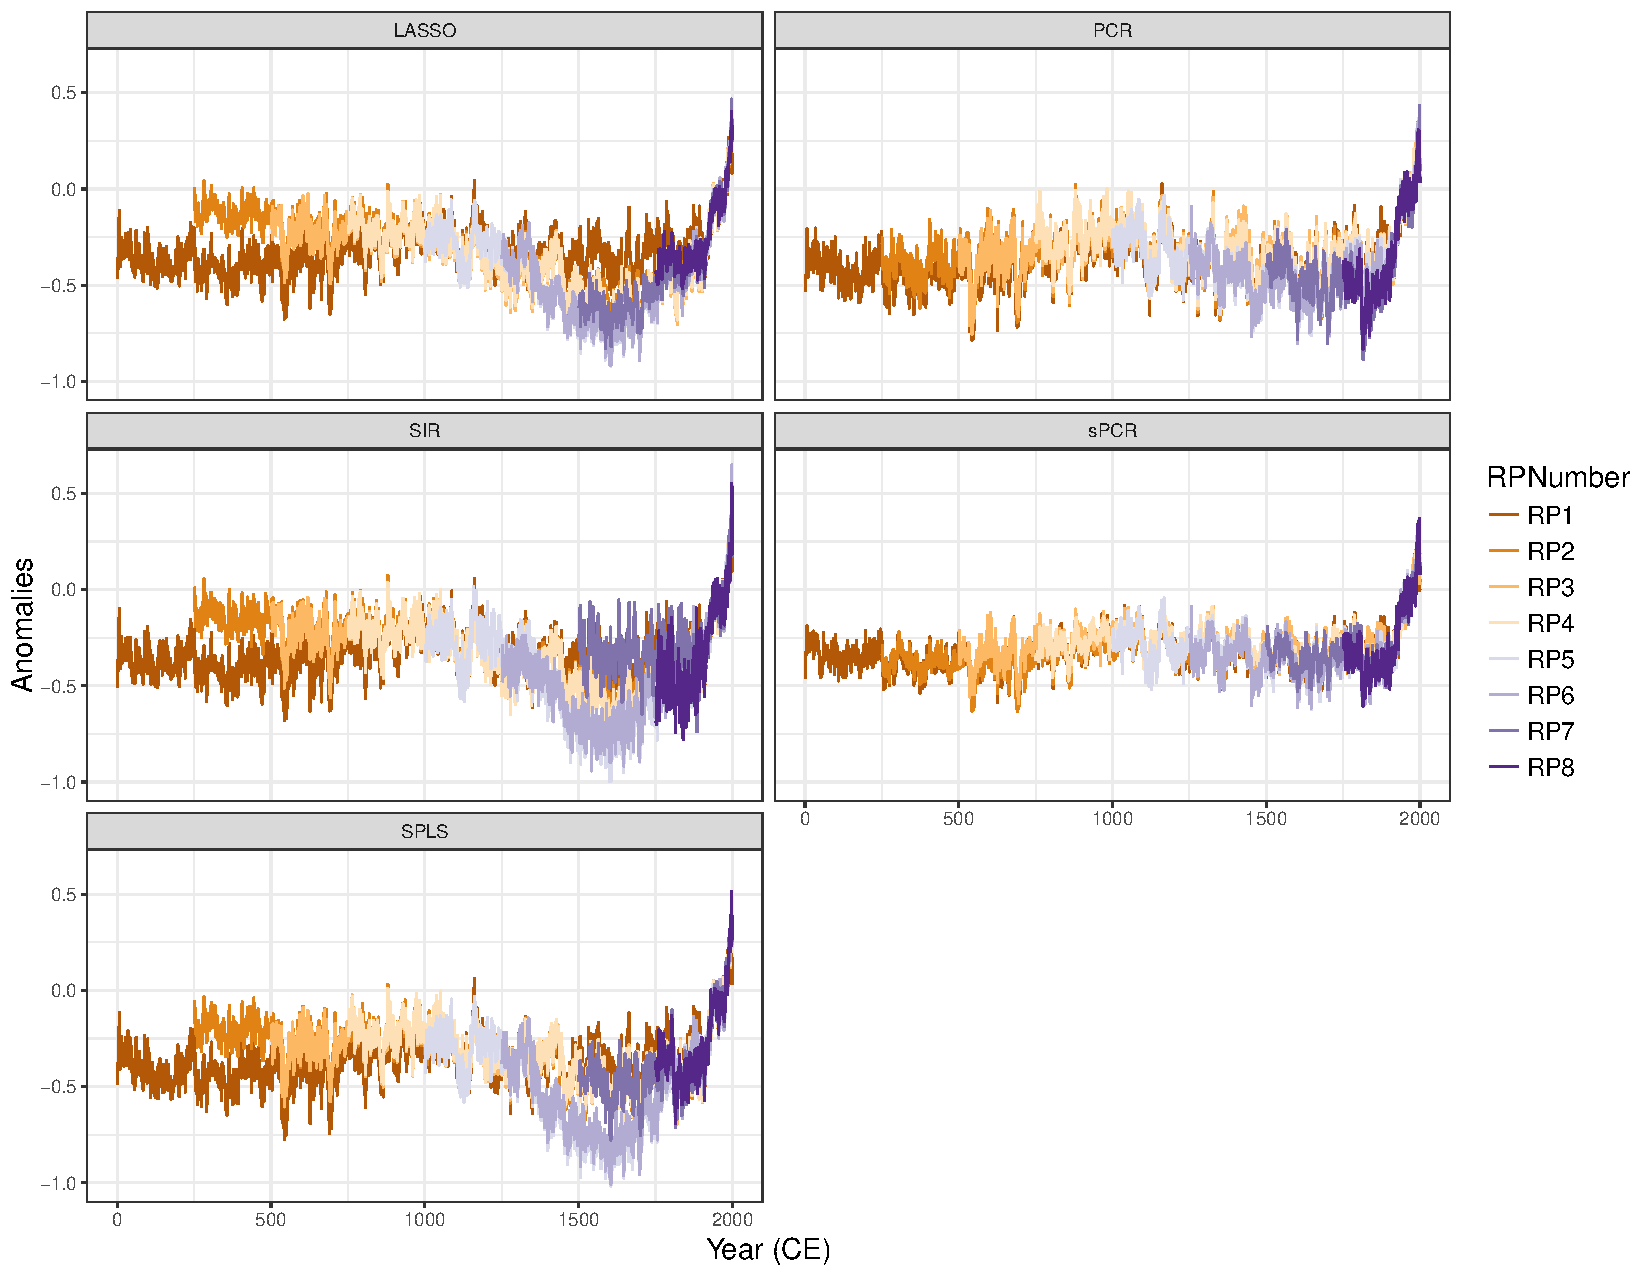
\includegraphics[scale=0.38]{RPs_type} 
  \caption{Reduced Proxies among methods.}
  \label{fig:RPs}
\end{figure}




An important aspect we notice from the distribution of Table
\ref{tab:distdate} is that the number of proxies can be greater or at least very
closed to the number of available observations in the calibration period defined as
1900-2000CE \footnote{The choice of the calibration period is based on the
  arguments shown in \cite{Barboza2014}} (101 observations), which can cause overfitting issues or
dimensionality problems in the use of classical linear models. Due to the above
reasons we investigated various data reduction techniques with the aim of establishing 
a reliable linear model between the observed anomalies and the corresponding proxies in
Table \ref{tab:distdate}, based on the data in the calibration
period. Many different data reduction methods have been developed. We will focus on below five popular ones:  
%(Description of the five methods including the basic idea, the unique feature, the pros and cons of the method)
\begin{description}
\item[Lasso Regression (LR)]
  The Lasso regression penalizes the usual sum of squares with an argument
 containing the sum of the absolute values of each coefficient in the classical
 linear regression model, multiplied by an additional smoothing parameter  (\cite{Tibshirani1996}). Due
 to the geometric nature of the term of penalization, the search of estimators
 tends to assign values very close to zero to variables that have almost null
 effects with respect to the dependent variable, which makes the resulting
 models easily interpretable. This method is very common to data reduction and easy to implement, but it often tends to select models with an excess of complexity, that is,
 it tends to show "false positives" in the variable selection process 
 (\cite{Fan2010}). Lasso could also run into inconsistency issues when the
 variables are highly correlated (\cite{Zou2005}).
 We used 10-fold cross validation to select the smoothing parameter when we carried out Lasso regression (see \cite{Tibshirani1996} and \cite{Friedman2010} for more details). 
\item[Sparse Partial Least Squares (sPLS)] 
  Partial least squares seek to reduce the high-dimensionality issues of the
  design matrix in  
  linear regression models through a latent matrix whose columns maximize
  \bl{can we replace the rest of the sentence by "their linear correlation with
    the responses"}\lb{I think it's better now}the 
  product of their linear correlation with the response and its
  variance. The sPLS method further introduces sparseness to the partial least squares
  estimators by means of a $L_1$-penalty with a thresholding parameter, in order to avoid inconsistency problems when there are a
  substantial number of noisy covariates (\cite{Chun2010} and
  \cite{Chung2013}). However, this method is inefficient in
  measuring the statistical significance of whether the parameters associated to certain
  variables are effectively zero (\cite{OlsonHunt2014}). In our implementation, the
  thresholding parameter involved in sPLS is estimated using a 10-fold cross-validation criteria.    
\item[Sliced Inverse Regression (SIR) with CSS selection method]
  In general, the SIR methods (\cite{Li1991},
  \cite{Duan1991}, \cite{Zhong2005}, \cite{Li2008}, \cite{Coudret2014}, \cite{Weisberg2002} among
  others) reduce the excess of dimension in a non-parametric setting through the
  estimation of the linear space spanned by the coefficients of the covariables,
  also known as \textit{effective dimension reduction} (EDR) subspace. 
  This subspace is obtained by an approximate eigenvalue decomposition that
  involves an estimation of the covariance matrices of the design matrix and
  the conditional expectation of the explanatory variables given the
  response. The
  estimation of the covariance matrix requires to partition the dependent variable into subgroups, called \textit{slices}.
  The SIR method can capture both linear or nonlinear associations between the response and
  covariates. However, the estimation of the dimension
  reduction space does not actually lead to a variable selection procedure and the
  covariance estimation relies heavily on the homogeneity of the response within
  each slice (\cite{Wu2010}). Because of this, we opt to incorporate the CSS
  (\textit{Closest submodel selection}) variable 
  selection procedure into the SIR method. Furthermore, to better deal with the fact that there is a larger number of
  covariates than observations, we employed the SIR-QZ algorithm, an upgrade of the SIR method based on the generalized Shur decomposition for undermined cases (\cite{Coudret2014} and \cite{Coudret2017}).   
  %\footnote{The SIR-QZ method is based on the generalized Shur decomposition and it aims to solve the eigenvalue problem of SIR for undetermined cases.} instead  (see \cite{Coudret2014} and \cite{Coudret2017}).
  %This compound method allows us to select
  %reduced models that are close to the complete model (possibly with excess
  %of dimension) in terms of their eigenvalue decompositions. 
  Finally, we studied the association between proxies and temperatures
  through a linear regression between the observed anomalies and a number of EDR directions, i.e., orthogonal basis of the EDR subspace, determined by marginal dimension tests (\cite{Cook2004}). 
\item[Principal Component Regression (PCR)]
PCR simply means that we replace the original covariates by their PCs. To select how many and which PCs to use, we fitted a regression model between the temperature and PCs of eight different sets of covariates selected in each of the eight different time periods based on the training data in calibration period. We then selected the number of PCs in each of
the eight regressions as the minimum number that attains, for the first time, an adjusted
$R^2$ of at least 70\% in each case. PCR is often used when covariates are
highly-correlated or when the number of covariates is larger than the number of 
 observations. A caveat of this method is that the principal components
with smaller contribution to variance are not necessarily the ones that
associate less with the dependent variable in a linear regression model (
\cite{Jolliffe1982} and \cite{Tibshirani1996}). 
\item[Supervised Principal Components (sPCR)]
Because of the above-mentioned caveat of directly using PCR, \cite{Bair2006} developed a technique where PCR is applied only
to a certain subset of covariates that exhibits a considerable amount of association
 with the dependent variable, and the threshold of ``considerable" is chosen through
cross-validation. Compared to PCR, the sPCR ensures the dimensionality
reduction on the covariates space while taking the association between
the covariates and the dependent variable into account. In general, its performance is quite similar to
sPLS method (\cite{Chung2013}).  
\end{description}

The data reduction allows us to fit linear regression models between temperatures and proxies. After we fit a linear regression model under each of the five data reduction methods and for each of the eight proxy groups listed in Table \ref{tab:distdate}, we further reduce the proxies into a single reduced proxy series following \cite{Barboza2014}. All reduced proxies are shown in Figure \ref{fig:RPs}.  These series are highly correlated, with the reduced proxies obtained by PCR standing out as least similar to the others by this metric (Fig.~\ref{fig:CorrRPs}).

\begin{figure}[H]
  \centering
 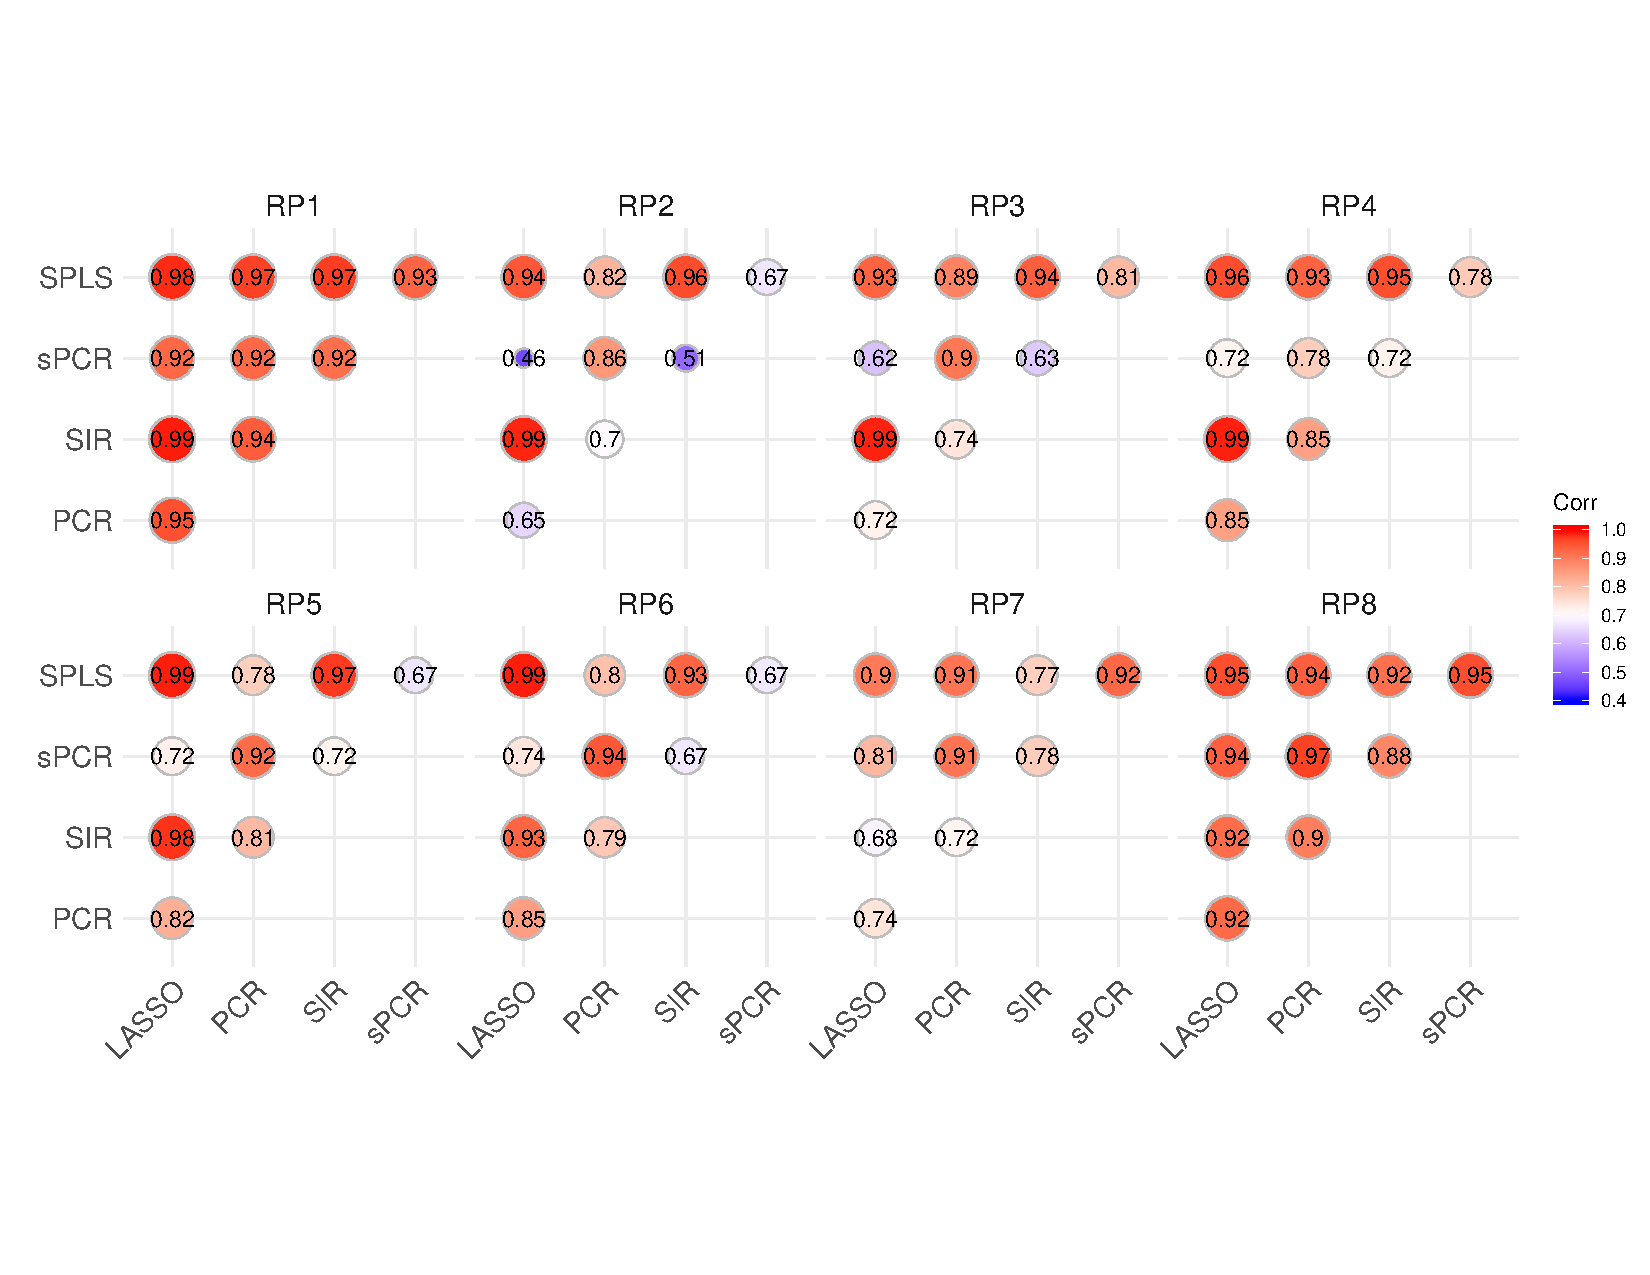
\includegraphics[scale=0.38]{CorMatrixRPs} 
  \caption{Correlation Matrices among 5 different Reduced Proxy series}
  \label{fig:CorrRPs}
\end{figure}

%Pba
%Pba2
%\section{Integrated Nested Laplace Approximation (INLA).}
%\label{sec:inla}

\subsection{Model Specification}
\label{sec:modelspec}
As we emphasized in the introduction, Bayesian hierarchical models (BHM) are very powerful tools and thus we will adopt this modeling framework for our problem. The first level of BHM is always designated for modeling the likelihood of data. In the second level, forcings are often included to improve
the reconstruction. However, reconstruction without forcings involved is more
desirable when we try to use proxy data to evaluate the climate models, because
in such case the forcings will introduce circularity issue\lb{Julien: can you
  add here more details about this circularity issue?}. We therefore will also
explore the model that substitutes forcings by a smooth function defined as a
linear combination of spline bases and a model composed by a combination of both
terms.
%The most popular model is to integrate all information using Bayesian
%hierarchical models.

Below we first define notations for our models:
%Our models are based on the one presented in \cite{Barboza2014}. Now we define some notation, %assuming that all the variables are set at time $t$.
\begin{itemize}
\item $RP_t^i$: $i$-th reduced proxy at time $t$.
  
\item $T_t$: temperature anomaly at time $t$.
  
\item $\tilde C_t = \log (C_t)$: Transformed greenhouse gases. The log
  transformation is chosen to approximate the radiative forcing due to changes
  in the equivalent CO$_2$ concentration. (\cite{Barboza2014})
  
\item $\tilde V_t = \log (-V_t+1)$: Transformed volcanic forcing. See more details in \cite{Barboza2014} for the choice of the transformation.
  
\item $B_t^{k,\tau}$: $k$-th B-Spline basis function at time $t$ with a uniform knot
  sequence $\tau$ (\cite{DeBoor2001} and \cite{Ramsay2005}). Here we choose
  cubic B-spline bases and we denote $K(\tau)$ as the total number of basis elements.  
\end{itemize}
We then define the first level of BHM as
\begin{align*}
RP_t^i=\alpha_0^i+\alpha_1^iT_t+\epsilon^i_t,  
\end{align*}
where $\{\alpha^i_j\}$ are random parameters for $i=1,\ldots,N$ and $j=0,1$,  $\epsilon^i_t$ are normally-distributed random variables with finite variances
$\{\sigma^2_i\}$. Note that in our case $N=8$, since we are working with 8
reduced proxies. The time variable $t$ is defined on each $RP$ according to the
time intervals of Table \ref{tab:distdate}. \bl{Are you defining random effects model? I don't see this
  is the case. Define what is N here? Since you have 8 time periods, the RP
  should have 8 segments, you concatenate them into one single series?}\lb{I
  changed the notation for the variances, now they don't seem random-effect
  variances. $N$ is defined and I explained how the time segments are chosen.}

The second level will be defined in three different forms depending on whether
forcings and/or BSplines will be included. We have
\begin{description}
\item[Model NF]
  \begin{align}\label{eq:M1}
    T_t=\beta_0+\sum_{k=1}^{K(\tau)}\beta_k B_t^{k,\tau}+\eta_t,
  \end{align}
where $\beta_k$ are coefficients for B-spline bases, and
$\eta_t$ are also normally-distributed random variables with finite variances
$\sigma^2_{\eta}$. For simplicity, the error terms $\epsilon^i_t$ and $\eta_t$
are assumed to be independent. The main idea of this model is to evaluate the
central hypothesis of this article, that is, the paleoclimate reconstruction can
perform  well without taking into account the external forcings, as long as a
smoothing function has been included to approximate the dynamic behavior of the
temperature series. In order to have a baseline model to evaluate Model NF, we
define
\item[Model WF]
  \begin{align}\label{eq:M2}
    T_t=\beta_0+\beta_1S_t+\beta_2\tilde V_t+\beta_3\tilde C_t+\eta_t.
  \end{align}
Both first level and second level models are defined for
$t=1,\cdots,2000$ (Common Era). \bl{should $t$ also include the calibration period?}\lb{Yes} It is important to add that in Models NF and WF we simply assume
an independent error structures. This is because \cite{Barboza2014} 
found that complex error structures make little difference when forcings are
added to the reconstruction.
\item[Model Mixed]
  This model is a combination of equations \eqref{eq:M1} and \eqref{eq:M2} as follows:
  \begin{align*}
    T_t=\beta_0+\beta_1S_t+\beta_2\tilde V_t+\beta_3\tilde C_t+\sum_{k=1}^{K(\tau)}\gamma_k B_t^{k,\tau}+\eta_t
  \end{align*}
  where $\gamma_k$ are the coefficients for the B-Spline basis in this case. \lb{Julien: please include an explanation why this model is interesting in the
    climatology community.}
\end{description}

\subsection{Sampling with INLA}

The computational challenge has been a concern for paleoclimate reconstructions using Bayesian methods. It is crucial to overcome this computational bottleneck before we can move forward to a more complex space-time reconstruction. Here we introduce the INLA sampling strategy to accelerate our global series reconstruction, and we hope this experiment can be served as a pioneer for employing INLA in other more complex reconstructions. 

%The computation is slow for even a global reconstruction, let alone a space-time reconstruction in our mind. We now introduce INLA to our reconstruction by adapting our model to the general specification of  the INLA framework. Now it is fast and we plan to extend this to space-time reconstruction. 

The INLA approach is applicable to a general specification for which the mean $\eta_i$ of  observations $y_i$ follows a  linear structure:
\begin{align}\label{eq:meanINLA}
  \eta_i = \alpha +\sum_{m-=1}^M\beta_mx_{mi}+\sum_{l=1}^Lf_l(z_{li})
\end{align}
where $\alpha$ represents an intercept, the coefficients
$\mathbf{\beta} = (\beta_1,\ldots,\beta_M)$ relate $M$ covariates
$(x_1,\ldots,x_M)$ to $\eta_i$, and $f = \{f_1(\cdot),\ldots,f_L(\cdot)\}$ is a collection of
random effects defined on a set of $L$ covariates $(z_1,\ldots,z_L)$ (see
\cite{Rue2009} and \cite{Blangiardo2013}). 
Denote the set of random variables as
$\theta = (\alpha,\beta,f)$ with $K$ hyperparameters $\psi =
\{\psi_1,\ldots,\psi_K\}$, and the vector of observations as $y=(y_1,\ldots,y_n)$. Model \eqref{eq:meanINLA} leads to conditional independence of $y$ given $\theta$ and $\psi$:
\begin{align*}
  p(y|\theta,\psi)=\prod_{i=1}^np(y_i|\theta_i,\psi).
\end{align*}
In our models, if we consider $y_i$ as the reduced proxies,  $\eta_i$ the
linear mean of the reduced proxies, $x_m$ the external forcings and/or the set
of spline basis, and $f(z_l)$ are the latent variables (temperature anomalies in
our case), then our models fall into the general specification of INLA. 


The main objectives of our Bayesian estimation are to compute the
marginal posterior distribution of each parameter in $\theta$:
\begin{align*}
  p(\theta_i|y) = \int p(\theta_i,\psi|y)d \psi = \int p(\theta_i|\psi,y)p(\psi|y)d \psi
\end{align*}
To attain computational advantages, INLA approach assumes that (i) the prior of vector $\theta$ is a multivariate normal random vector with a precision matrix that depends on hyperparameters $\psi$, and (ii) the vector
$\theta$ is conditionally independent given the hyperparameters. These two
assumptions specify $\theta$ as a Gaussian Markov random field. INLA further 
substitutes the two components $p(\psi|y)$ and $p(\theta_i|\psi,y)$ by their approximations. The first component can be approximated using a
Laplace Approximation (see \cite{Tierney1986}):
\begin{align*}
  p(\psi|y)&=\frac{p(\theta,\psi|y)}{p(\theta|\psi,y)}\propto \frac{p(\psi)p(\theta|\psi)p(y|\theta)}{p(\theta|\psi,y)}\\
           & \approx  \frac{p(\psi)p(\theta|\psi)p(y|\theta)}{\tilde p(\theta|\psi,y)} \Biggm |_{\theta=\theta^*(\psi)} := \tilde p(\psi|y),
\end{align*}
where $\tilde p(\theta|\psi,y)$ is the Gaussian approximation of
$p(\theta|\psi,y)$ and $\theta^*(\psi)$ is its mode (see \cite{Rue2009}). The
second component can be approximated in a similar way:
\begin{align}\label{eq:second}
  p(\theta_i|\psi,y)&=\frac{p((\theta_i,\theta_{-i})|\psi,y)}{p(\theta_{-i}|\theta_i,\psi,y)} \notag \\
  &\approx \frac{p((\theta_i,\theta_{-i})|\psi,y)}{\tilde p(\theta_{-i}|\theta_i,\psi,y)} \Biggm |_{\theta_{-i}=\theta_{-i}^*(\theta_i,\psi)}:=\tilde p(\theta_i|\psi,y),
\end{align}
where $\theta=(\theta_i,\theta_{-i})$, $\tilde p(\theta_{-i}|\theta_i,\psi,y)$ is the Gaussian approximation of
$p(\theta_{-i}|\theta_i,\psi,y)$ and $\theta_{-i}^*(\theta_i,\psi)$ is its mode,  
The approximation in \eqref{eq:second} possesses good precision, but it is very time demanding because it
requires to recompute $\tilde p(\theta_i|\psi,y)$ for each value of $\theta$ and $\psi$. A
more efficient approach is to use the simplified Laplace Approximation that is
based on a Taylor's expansion of $\tilde p(\theta_i|\psi,y)$ in 
\eqref{eq:second}. As mentioned in \cite{Rue2009} and \cite{Blangiardo2013},
INLA first explores the marginal joint posterior of the hyperparameters $\tilde
p(\psi | y)$ in order to locate the mode and then performs a grid search to 
produce a set of ``relevant'' points $\{\psi^*\}$ together with a set of weights
$w_{\psi^*}$ as an approximation of this marginal distribution. The marginals
$p(\psi^*|y)$ are then refined using interpolation methods. Finally, the marginals
$\tilde p(\theta_i|y)$ are obtained as follows:
\begin{align*}
  \tilde p(\theta_i|y) \approx \sum_{\psi^*}\tilde p(\theta_i|\psi^*,y)\tilde p(\psi^*|y)w_{\psi^*}.
\end{align*}

\subsection{Priors}
The models proposed in section \ref{sec:modelspec} were
implemented using the R package \textbf{r-inla}\footnote{www.r-inla.org}. The
implementation followed the methods provided in \cite{Ruiz-Cardenas2012} and
\cite{Muff2015} on the use of the INLA methodology in state-space models,
dynamic linear models, and in general models whose mean can be written
into equation \eqref{eq:meanINLA}. These
methods together with \cite{Martins2013} allow INLA to be applicable to a wide array of Bayesian models such as BHM that consists of several layers. 

As Bayesian estimation, INLA requires priors for unknown parameters. Below is the list of priors we used in our models:
\begin{itemize}
\item $\alpha^i_j\sim N(0,3)$, $\beta_\ell \sim N(0,3)$ for $i=1,\ldots,N$, $j=0,1$, and  $\ell=0,\ldots,3$
  for Model WF and $\ell=0,\ldots,K(\tau)$ for Model NF. The choice of the variance is
  completely arbitrary, but the main idea is to select a relatively large one.
  
\item $\rho_i := -\log \sigma^2_{\epsilon^i}\sim \text{log-gamma}(1,10^{-20})$
  (very small precision) for $i=1,\ldots,N$.
  
\item $\rho_0 := -\log \sigma^2_\eta \sim \text{log-gamma}(1,10^{-20})$ (very
  small precision).
\end{itemize}


\section{Results.}
\label{sec:results}
\subsection{Impact of the number of reduced proxies and the reduction method}
As a first exercise, we analyze the change in the predictive capacity of the
reconstruction model when more equations involving proxies are included. We used
two scoring rules in \cite{Gneiting2007a} as measures of predictive ability:
IS$_\alpha$ (Interval Score at $\alpha$ level) and CRPS (Continuous Ranked
Probability Score). These scores have been previously employed in the
verification of point forecasts in environmental sciences for example, as well as the area
of paleoclimatic reconstructions (see \cite{Barboza2014} and
\cite{Scheuerer2014}). Table \ref{tab:comparisontot} contains the predictive
measures using the INLA's prediction intervals and: (1) the \textbf{observed
  anomalies} over 1850-1899 as an out-of-sample validation interval and (2) the borehole-based
reconstruction of \cite{Pollack2004} over 1500-1899 as an out-of-sample
validation interval. We compared in this case Model WF with a single RP
(the longest available) with respect to model WF using the 8 available reduced
proxies, where the comparison was made under the five dimension reduction
methods explained above.

\begin{table}
\centering
\begin{tabular}{lll|rrr|rrr}
  \toprule
    \multicolumn{3}{c}{} & \multicolumn{3}{|c}{Observed Anomalies}  & \multicolumn{3}{|c}{PS04 dataset} \\
  \midrule
  \textbf{Model} & $N$ & \textbf{Method} & IS$_{80}$ & IS$_{95}$ & CRPS & IS$_{80}$ & IS$_{95}$ & CRPS  \\ 
  \midrule
  WF & 1 & PCR & 0.4678 & 0.1792 & 0.1641 & 0.5422 & 0.1792 & 0.2770 \\ 
  WF & 1 & sPCR & 0.5821 & 0.2146 & 0.2593 & 0.6595 & 0.2147 & 0.3299 \\ 
  WF & 1 & LASSO & 0.4658 & 0.1780 & 0.1655 & 0.5462 & 0.1780 & 0.2913 \\ 
  WF & 1 & SPLS & 0.4749 & 0.1813 & 0.1810 & 0.5504 & 0.1812 & 0.2887 \\ 
  WF & 1 & SIR & 0.4779 & 0.1819 & 0.1671 & 0.5509 & 0.1818 & 0.2881 \\
  \midrule
  WF & 8 & PCR & 0.2493 & 0.0840 & 0.0986 & 0.3802 & 0.1134 & 0.1617 \\ 
  WF & 8 & sPCR & 0.1969 & 0.0719 & 0.0745 & 0.6900 & 0.2468 & 0.2455 \\ 
  WF & 8 & LASSO & 0.5044 & 0.3128 & 0.1559 & 1.5297 & 1.2913 & 0.4153 \\ 
  WF & 8 & SPLS & 0.3436 & 0.1687 & 0.1177 & 1.3822 & 1.1036 & 0.3847 \\ 
  WF & 8 & SIR & 0.6485 & 0.4797 & 0.1871 & 1.7658 & 1.5793 & 0.4671 \\
  \midrule
  NF & 8 & PCR & 0.2966 & 0.0958 & 0.1249 & 0.3224 & 0.1026 & 0.1399 \\ 
  NF & 8 & sPCR & 0.4275 & 0.1624 & 0.1600 & 0.4272 & 0.1624 & 0.1505 \\ 
  NF & 8 & LASSO & 0.5434 & 0.3545 & 0.1644 & 1.5906 & 1.3666 & 0.4285 \\ 
  NF & 8 & SPLS & 0.2617 & 0.0942 & 0.0967 & 1.1900 & 0.8772 & 0.3433 \\ 
  NF & 8 & SIR & 0.5772 & 0.3955 & 0.1720 & 1.6679 & 1.4583 & 0.4459 \\
  \midrule
  Mixed & 8 & PCR & 0.3509 & 0.1101 & 0.1579 & 0.3233 & 0.1120 & 0.1338 \\ 
  Mixed & 8 & sPCR & 0.3660 & 0.1368 & 0.1357 & 0.3634 & 0.1368 & 0.1375 \\ 
  Mixed & 8 & LASSO & 0.5291 & 0.3385 & 0.1613 & 1.5672 & 1.3377 & 0.4234 \\ 
  Mixed & 8 & SPLS & 0.3131 & 0.1404 & 0.1101 & 1.3198 & 1.0284 & 0.3713 \\ 
  Mixed & 8 & SIR & 0.5986 & 0.4209 & 0.1766 & 1.7001 & 1.4973 & 0.4530 \\ 
   \bottomrule
\end{tabular}
  \caption{Comparison of predictive measures.}
  \label{tab:comparisontot}
\end{table}


% \begin{table}
%   \centering
%   \begin{tabular}{lll|rrr|rrr}
%     \toprule
%     \multicolumn{3}{c}{} & \multicolumn{3}{|c}{In-sample}  & \multicolumn{3}{|c}{Out-of-sample} \\
%     \midrule
%     \textbf{Model} & $N$ & \textbf{Method} & IS$_{80}$ & IS$_{95}$ & CRPS & IS$_{80}$ & IS$_{95}$ & CRPS \\
%     \midrule
%    SSwF & 1 & PCR & 0.4702 & 0.1799 & 0.1827 & 0.4678 & 0.1792 & 0.1641 \\ 
%    SSwF & 1 & sPCR & 1.1464 & 0.3635 & 0.4700 & 0.5821 & 0.2146 & 0.2593 \\ 
%    SSwF & 1 & LASSO & 0.4665 & 0.1786 & 0.1631 & 0.4658 & 0.1780 & 0.1655 \\ 
%    SSwF & 1 & SPLS & 0.4750 & 0.1817 & 0.1844 & 0.4749 & 0.1813 & 0.1810 \\ 
%    SSwF & 1 & SIR & 0.4763 & 0.1822 & 0.1736 & 0.4779 & 0.1819 & 0.1671 \\
%    \midrule
%    SSwF & 8 & PCR & 0.2166 & 0.0828 & 0.0727 & 0.2493 & 0.0840 & 0.0986 \\ 
%    SSwF & 8 & sPCR & 0.1935 & 0.0719 & 0.0722 & 0.1969 & 0.0719 & 0.0745 \\ 
%    SSwF & 8 & LASSO & 0.3382 & 0.1994 & 0.1103 & 0.5044 & 0.3128 & 0.1559 \\ 
%    SSwF & 8 & SPLS & 0.2669 & 0.1294 & 0.0945 & 0.3436 & 0.1687 & 0.1177 \\ 
%    SSwF & 8 & SIR & 0.4110 & 0.2845 & 0.1250 & 0.6485 & 0.4797 & 0.1871 \\
%    \midrule 
%    SSnF & 8 & PCR & 0.2496 & 0.0954 & 0.0820 & 0.2966 & 0.0958 & 0.1249 \\ 
%    SSnF & 8 & sPCR & 0.6757 & 0.2082 & 0.2715 & 0.4275 & 0.1624 & 0.1600 \\ 
%    SSnF & 8 & LASSO & 0.3569 & 0.2210 & 0.1143 & 0.5434 & 0.3545 & 0.1644 \\ 
%    SSnF & 8 & SPLS & 0.2230 & 0.0938 & 0.0843 & 0.2617 & 0.0942 & 0.0967 \\ 
%    SSnF & 8 & SIR & 0.3754 & 0.2426 & 0.1180 & 0.5772 & 0.3955 & 0.1720 \\
%    \bottomrule
% \end{tabular}
%   \caption{Comparison of predictive measures.}
%   \label{tab:comparisontot}
% \end{table}


It is evident that there is an improvement in all the measures when we use all the available reduced proxies over the case
$N=1$, under the methods SPLS, PCR and sPCR for the first validation period.
However, for the PS04 dataset validation, only
the PCR method shows an improvement in terms of measures.  Also note that, among the models with external forcings, the techniques that
guarantees better results in terms of prediction are sPCR and PCR.

\subsection{Impact of modeling assumptions}
We are also interested in assessing whether a linear combination of B-splines can model GMST without the inclusion of external
forcings at all. It is clear from equation \eqref{eq:ssnf} that one of the drawbacks of Model 2 is the arbitrariness of $K(\tau)$. We analyze the
relationship between the temperature observed during the calibration period
(1900-2000) and a linear combination of BSplines. The number of elements of the
base is selected according to the adjusted $R^2$ of a linear regression model between observed anomalies and
the corresponding basis elements. Based on the above, we selected 6
BSpline terms for this period and we take $K(\tau)=120$ based on the
assumption that the number of BSpline terms is uniform
throughout all the reconstruction period \jeg{this assumption seems strange given that the number of proxies varies drastically. Can you justify it?}. Finally we fit the model in
\eqref{eq:ssnf} with the previous choice of $K(\tau)$ using the five different RPs (section \ref{sec:rp}). These results are
shown in the last five rows of Table \ref{tab:comparisontot}. Due to the comments of the above paragraph, we opt to
use all the reduced proxies in this case. \jeg{I don't understand this sentence}
% Therefore, for each of
% the methods in section 4.1, the IS and CRPS measures were calculated for a fixed
% value of $K(\tau)$ over a grid defined in [1,50]. After this, the best $K(\tau)$
% for each method was selected using the IS and CRPS measures. These results are
% shown in the last four lines in Table \ref{tab:comparisontot}. Due to the comments of the above paragraph, we opt to
% use all the reduced proxies in this case.
% \begin{table}
%   \centering
%   \begin{tabular}{c|rrr}
%   \toprule
% Method  & IS$_{80}$ & IS$_{95}$ & CRPS \\ 
%   \midrule
% PCR & 0.1583 & 0.0532 & 0.0435 \\ 
%   LASSO & 0.1881 & 0.0640 & 0.0697 \\ 
%   SPLS & 0.1819 & 0.0611 & 0.0574 \\ 
%   SIR & 0.1649 & 0.0550 & 0.0462 \\ 
%    \bottomrule
% \end{tabular}
%   \caption{Comparison of predictive measures of Model 2.}
%   \label{tab:comparison2}
% \end{table}
Note that the SPLS method achieves a better performance in terms of all the
predictive measures for both validation periods, even though the PCR results
differ very little in its corresponding measures. 

In order to illustrate the reconstruction that we obtained for both models, we
considered the best four choices in terms of the validation measures in Table
\ref{tab:comparisontot}. sPCR and PCR methods for the SSwF model and SSPLS and
PCR for
the SSnF model are the best choices. First note that the four respective reconstructions of the
temperature anomalies in the Common Era are shown in
Figure \ref{fig:paleoCE1}.
\begin{figure}
  \centering
  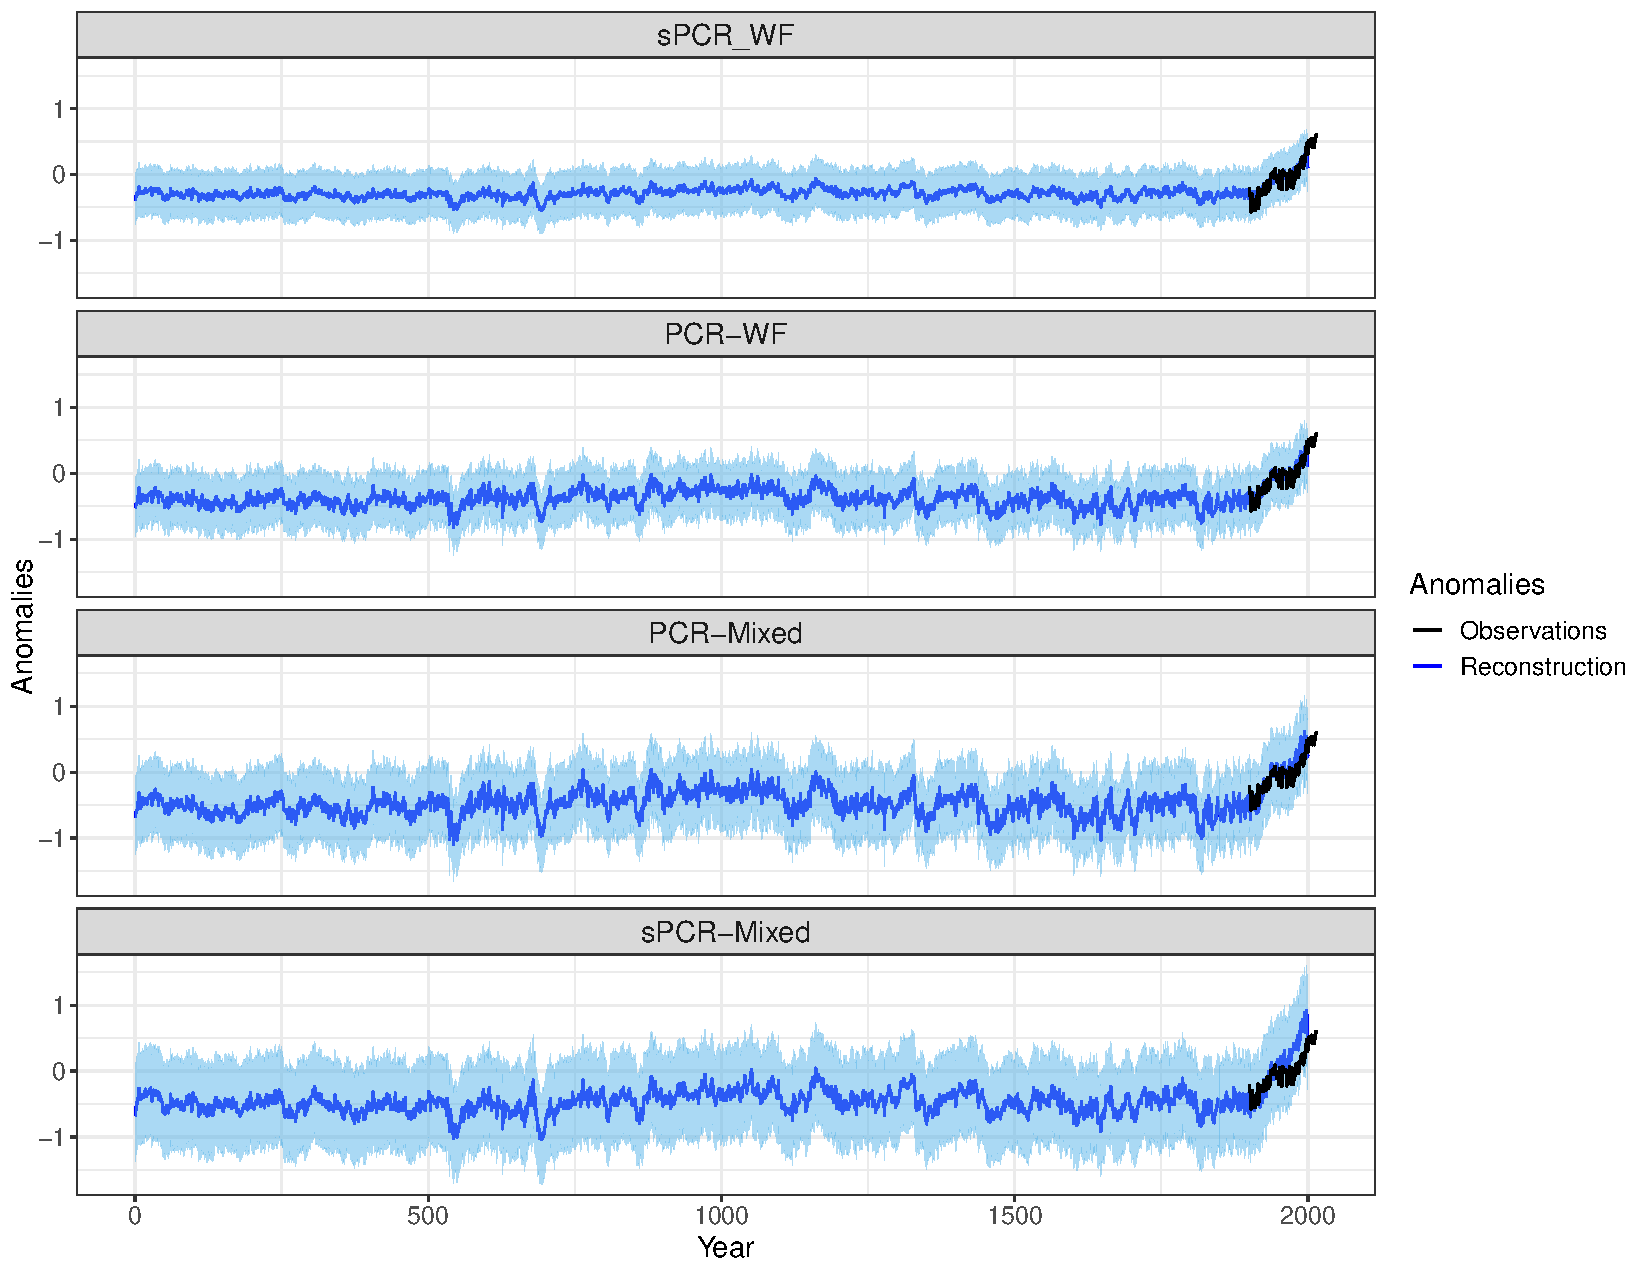
\includegraphics[scale=0.55]{RecCE_Final}
  \caption{Paleoclimate Reconstruction in the Common Era (CE) with 95\%
    prediction bands. Best two choices per validation method.}
  \label{fig:paleoCE1}
\end{figure}

\jeg{I take issue with the definition of "best" here. This is entirely contingent on the choice of calibration and verification period, and many studies have shown that you can obtain different results with different defintions of such periods. This is basically a cross-validation exercise, and there would be many different choices (5-fold cross validation is my personal favorite). I would strongly urge against declaring any ``best'' choices based only on the short observational record. Inevitably we need to assert our favorites, but let us not fool ourselves that this is an objective choice.}

The best choice (sPCR-SSwF) shows an interesting
balance in terms of the variance of the reconstructed series and the width of
the confidence region approximated by INLA. Reconstructions PCR-SSwF and
PCR-SSnF show similar small-scale tendencies with respect to the best choice, but the width of their confidence regions
is greater, which is an indicator of less precision in the overall
reconstruction. These last reconstructions also have smaller amplitude than the one shown by the best
option, this clearly is an indicator that the absence or presence of the
forcings is not decisive at the time of performing the reconstruction. In
general terms these three reconstructions have a very similar average level
of anomalies, except that the PCR-SSnF method gives anomalies that are generally a
bit colder than the two best ones. A closer look of the best reconstructions is shown in Figure
\ref{fig:paleo19001}.
\begin{figure}
  \centering
  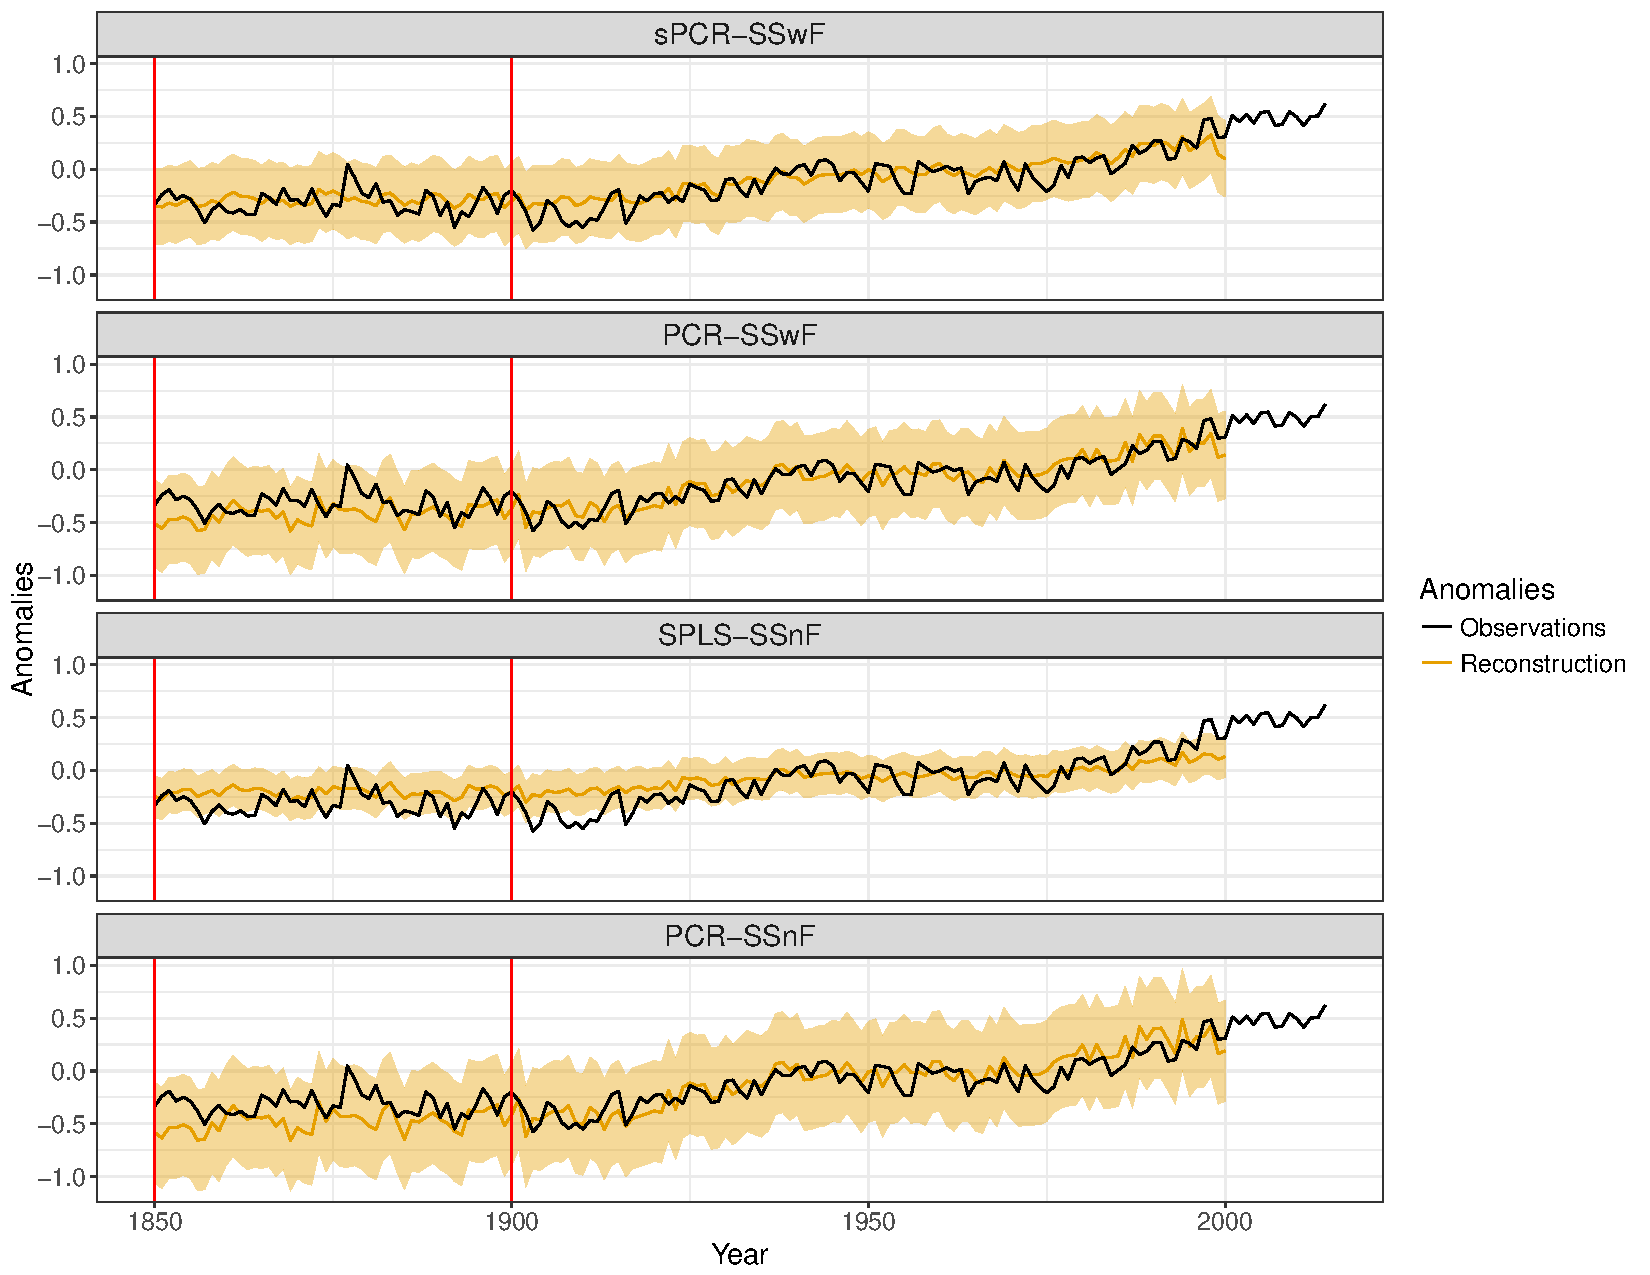
\includegraphics[scale=0.55]{Rec1900_Final}
  \caption{Paleoclimate Reconstruction 1850-2000 with 95\%
    prediction bands. Best two choices per validation method. The out-of-sample validation period is
    located between the red lines.}
  \label{fig:paleo19001}
\end{figure}
Note that although the reconstruction we obtained in
SPLS-SSnF has a fairly narrow confidence region, there are quite a few observed
anomalies during the out-of-sample testing period (1850-1899) that are outside
this range within the calibration period as well as the beginning of the 20th
century. In addition, this reconstruction has smaller variance that the observed
anomalies during both validation periods, which is not so noticeable in the other
three best reconstructions and  it also overestimates the the observed series
during the out-of-sample validation period. On the other hand, the reconstructions PCR-SSwF and PCR-SSnF  
underestimate the observed anomalies considerably during the period 1850-1900,
although the observed series during this period is completely contained in the
respective confidence bands. For the above reasons we believe that the
reconstruction that has the best results is the one obtained by sPCR-SSwF, followed
by the PCR-SSwF model. 

\begin{figure}
  \centering
  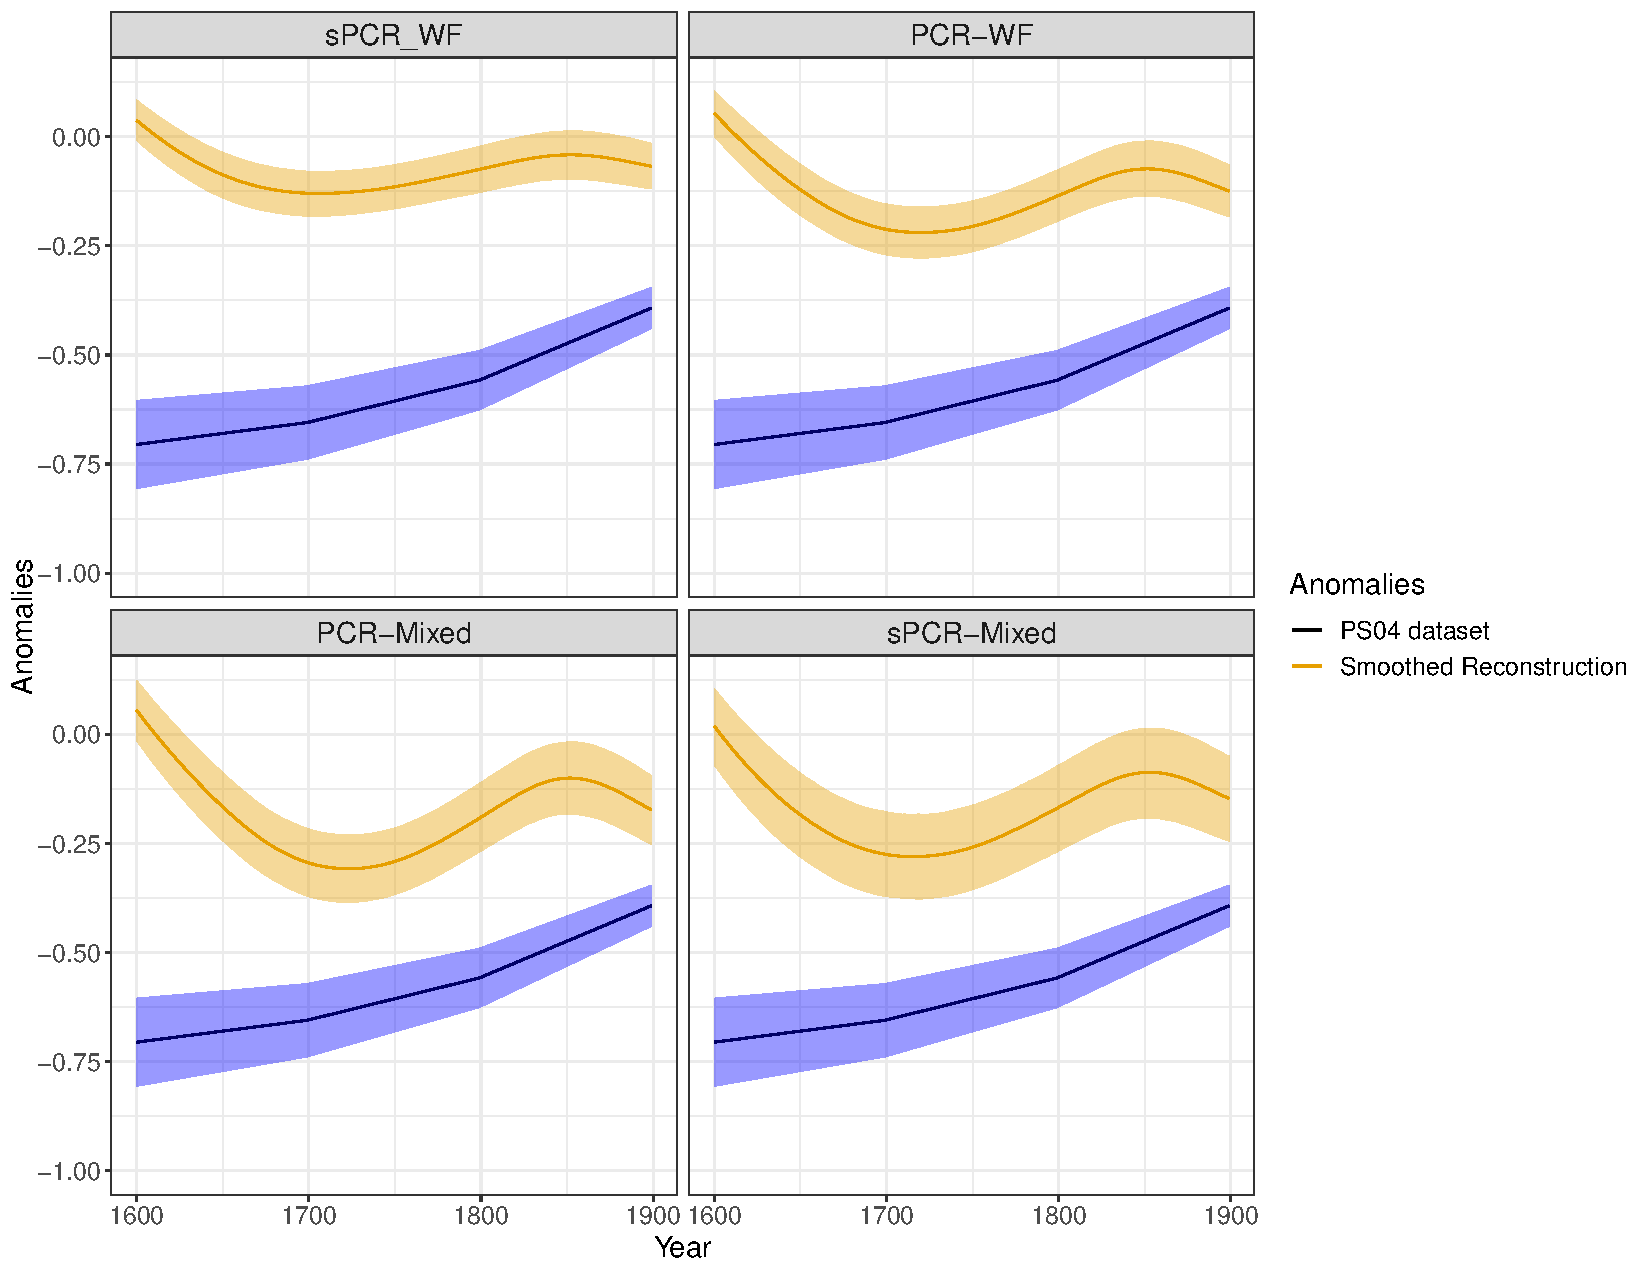
\includegraphics[scale=0.55]{Rec1500_Final}
  \caption{Paleoclimate Reconstruction 1500-2000 with 95\%
    prediction bands. Best two choices per validation method. The out-of-sample validation period is
    located between the red lines.}
  \label{fig:paleo15001}
\end{figure}

\subsection{Impact of Laplace approximations}

\jeg{I think this is what you're trying to do here, but I can't be sure...}

The SSwF model in its simplest case (1 proxy) was fitted in \cite{Barboza2014}
using an MCMC approach. We employed this approach in order to adjust the
SSwF model with the first reduced proxy from the sPCR method (the best choice
obtained from Table \ref{tab:comparisontot}). The MCMC was performed using the
same priors as in \cite{Barboza2014}, but with a larger calibration period
(1900-2000). The results are shown in Figures \ref{fig:paleoCE4} and
\ref{fig:paleo19004} in the appendix, together with the results of the best
model according to Table \ref{tab:comparisontot}. Note that the MCMC reconstruction is cooler than INLA's, due
mainly to the inclusion of more information from the remaining 7 reduced
proxies. The MCMC confidence bands along the reconstruction period are narrower,
this can be an indicator that the whole reconstruction obtained through a MCMC technique has larger
bias than the one obtained with INLA method. During the out-of-sample validation
period we can be observe that the reconstruction using the MCMC method
underestimates the observed anomaly considerably, while in the case of INLA that
does not happen at all. In addition, the validation measures IS$_{80}$ and IS$_{90}$
during the same period are 0.3 and 0.16 respectively for the MCMC case, and they
differ a lot with respect to the ones obtained for the best model in Table
\ref{tab:comparisontot}. It is clear then that the adjustment outside the
calibration period is not the most optimal according to this method. We can
compare also these two models in terms of the estimated coefficients of the
external forcings in equation \eqref{eq:sswf}. The estimated density function
for each coefficient is shown in Figure \ref{fig:betas}. Note that the INLA's
estimates are more precise and their magnitude are quite similar for the Solar and Vulcanism
forcings. The greenhouse-gases coefficient is significantly smaller than the one
obtained in the MCMC model, mainly due to a larger effect of the remaining
reduced proxies on the reconstruction, but in general, this external forcings
represents the one with greatest weight when we describe the mean behavior of the anomalies.

In terms of computational efficiency the INLA procedure is quite remarkable, not only
for our case but in most of the previous works on the topic (see \cite{Rue2009},
\cite{Blangiardo2013}, \cite{Ruiz-Cardenas2012} for a few examples). The
computational time of an MCMC method was
aproximately 14 hours, whereas the computational time of INLA's best model with
8 RPs (most complex model) was aproximately 11 minutes \footnote{This comparison
was performed on an Ubuntu 16.04 server with Intel Xeon E5-2630 (8-cores,
2.40GHz) and 64 GB of RAM.}. 



% The same can be said
% for a closer look of the reconstructions during the period 1900-2000 (see
% . For comparison purposes,
% we also include the reconstructions of Model SSwF with the PCR method (see the
% upper panels of 
% figures ), where the
% main difference corresponds to the period 1-250 in terms of the variance of the
% mean function, mainly due to the sensitivity of the B-Spline basis to
% discrepancies among reduced proxies in a fixed time period. Also note that the
% resulting posterior densities of the external forcings (see Figure
% \ref{fig:betas} in the Appendix) suggest that both $S_t$
% and $\tilde C_t$ are quite significant to explain the temperature anomalies.    




% Finally, we also compare the nature of the linear function that determines the
% mean behavior of the state equation in both models. As the coefficients that
% accompany the covariates are random (External forcings for Model SSwF, B-Splines
% for Model SSnF) then it is possible to calculate confidence bands for the mean
% function in both cases. This is illustrated in Figure \ref{fig:meanfunction}.
% \begin{figure}
%   \centering
%   \includegraphics[scale=0.4]{MeanFunction_comp}
%   \caption{Mean function of the state equation and its 95\% confidence band.}
%   \label{fig:meanfunction}
% \end{figure}
% Note that the variance and the stability of the mean function are much greater
% in the best case of Model SSnF than in the best case of Model SSwF. This could be an
% indicator that Model SSwF has a greater bias in its mean behavior, which is a
% negative aspect in the reconstruction as a whole.




\section{Conclusions.}
\label{sec:conclusions}

A brief summary of what this paper did and what are the conclusions. 

Discuss about using INLA for space-time reconstruction...


%\printbibliography

\bibliographystyle{plain}
\bibliography{biblioteca}


\newpage
\appendix

\section{Additional Plots}
\jeg{most of these plots were essential to the paper, so I moved them to the main text}


% \begin{figure}[H]
%   \centering
%   \includegraphics[scale=0.4]{PAGES_composites_PCR5} 
%   \caption{Reduced Proxies using PC regression.}
%   \label{fig:proxiespcr}
% \end{figure}

\begin{figure}[H]
  \centering
  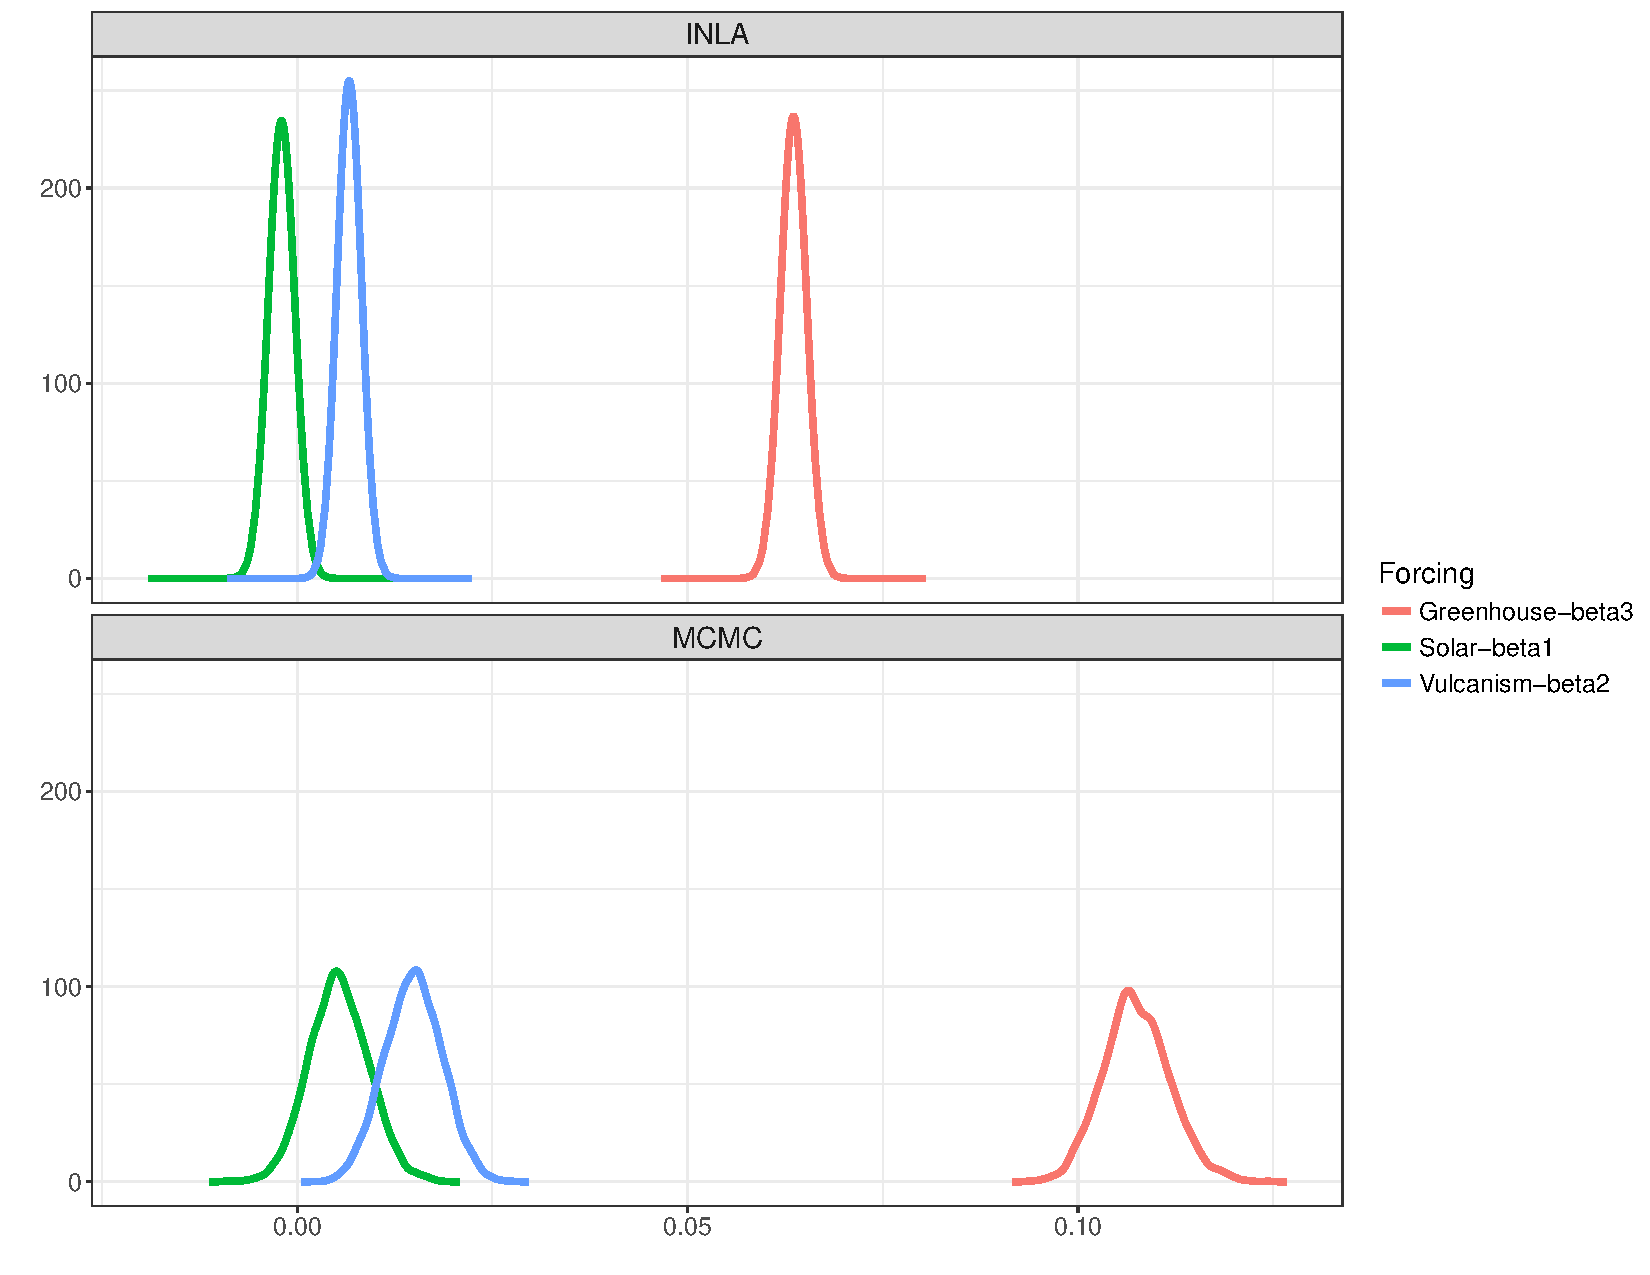
\includegraphics[scale=0.45]{PlotBetas}
  \caption{Posterior densities of $\beta_1$, $\beta_2$ and $\beta_3$ for Model
    sPCR-SSwF and MCMC using PCR single reduced proxy.}
  \label{fig:betas}
\end{figure}

% \begin{figure}[H]
%   \centering
%   \includegraphics[scale=0.35]{RecCE_PCR_Splines}
%   \caption{Paleoclimate Reconstruction in the Common Era (CE) with 95\%
%     prediction bands. PCR Method - Model 2.}
%   \label{fig:paleoCE3}
% \end{figure}

% \begin{figure}[H]
%   \centering
%   \includegraphics[scale=0.4]{Rec1900_PCR_Splines}
%   \caption{Paleoclimate Reconstruction 1900-2000 with 95\%
%     prediction bands. PCR Method - Model 2.}
%   \label{fig:paleo19003}
% \end{figure}

\begin{figure}[H]
  \centering
  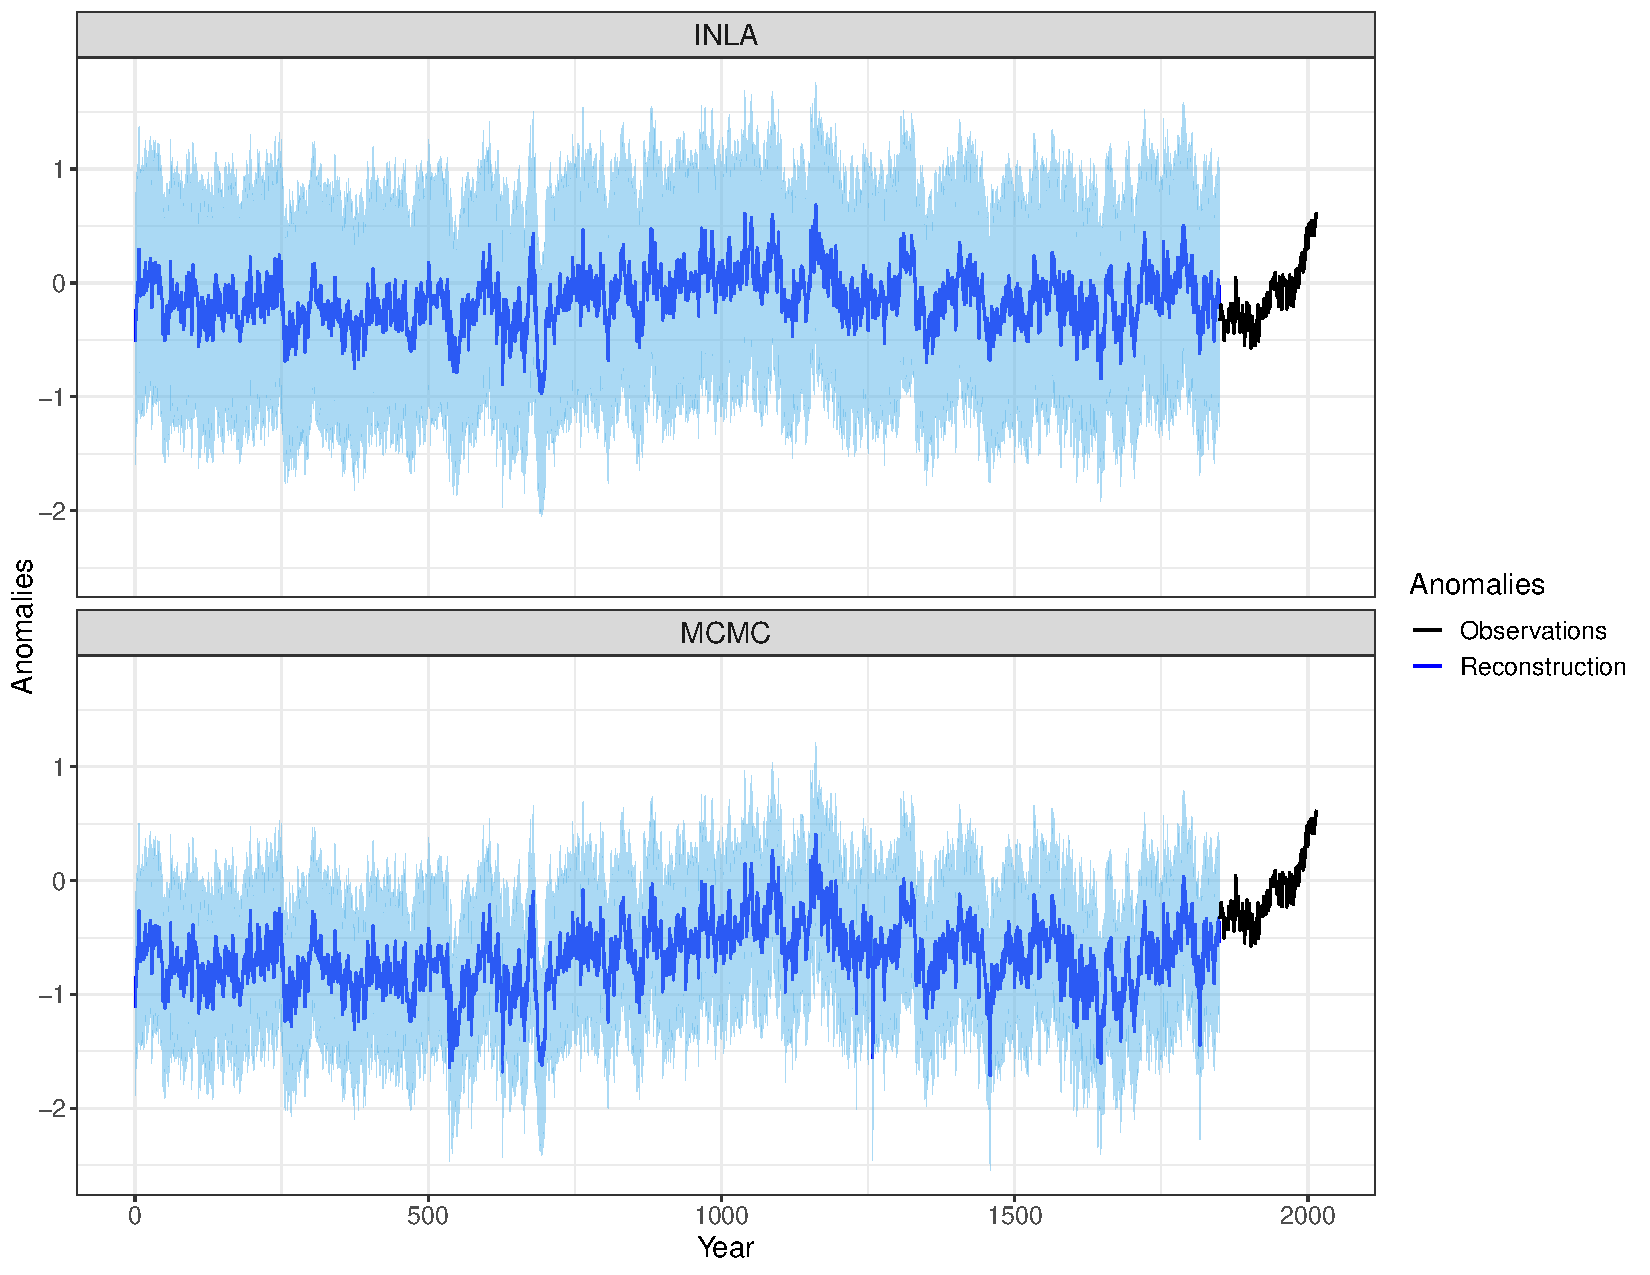
\includegraphics[scale=0.35]{RecCE_MCMC}
  \caption{Paleoclimate Reconstruction in the Common Era (CE) with 95\%
    prediction bands. Model sPCR-SSwF under two methods: INLA and MCMC.}
  \label{fig:paleoCE4}
\end{figure}

\begin{figure}[H]
  \centering
  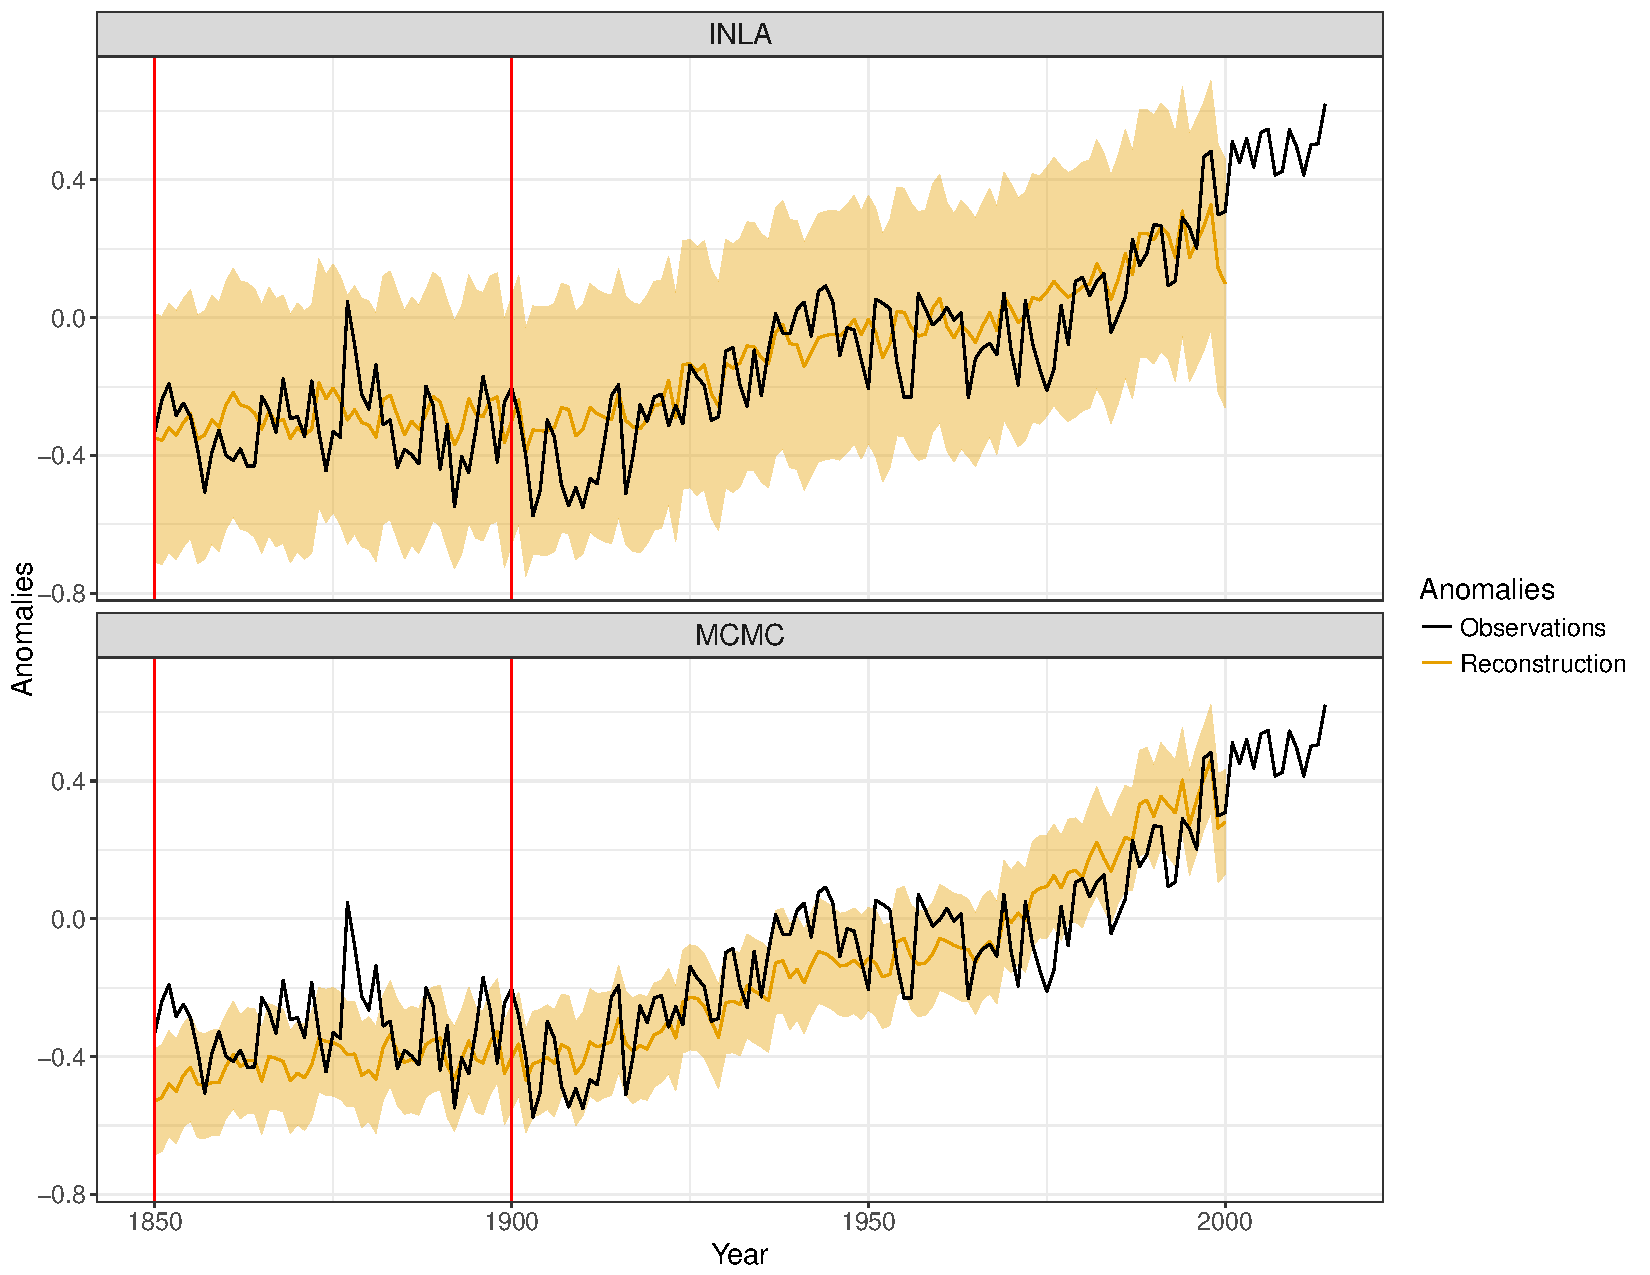
\includegraphics[scale=0.35]{Rec1900_MCMC}
  \caption{Paleoclimate Reconstruction 1900-2000 with 95\%
    prediction bands. Model sPCR-SSwF under two methods: INLA and MCMC.}
  \label{fig:paleo19004}
\end{figure}

\begin{figure}[H]
  \centering
  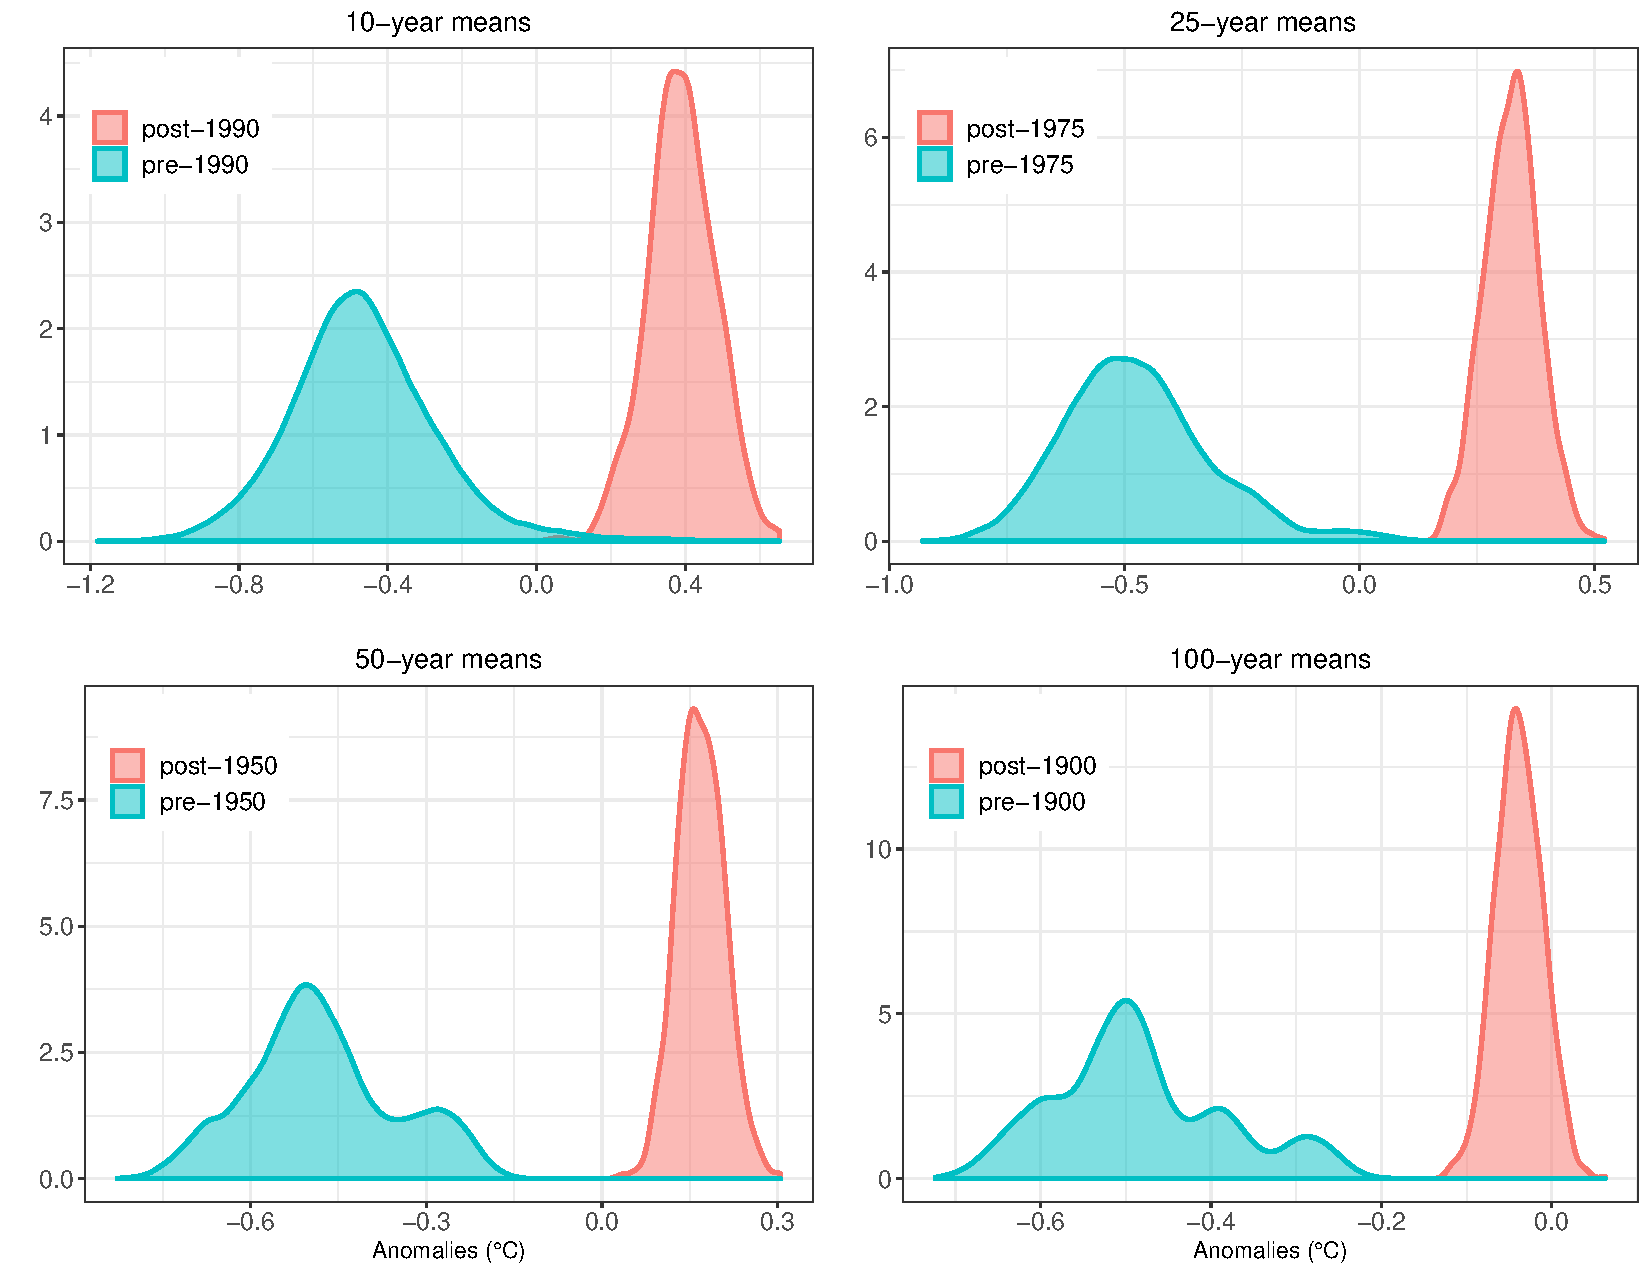
\includegraphics[scale=0.35]{compMeans}
  \caption{Comparison of the distribution of reconstructed anomalies for different time horizons. Model sPCR-SSwF.}
  \label{fig:compmeans}
\end{figure}

\begin{figure}[H]
  \centering
  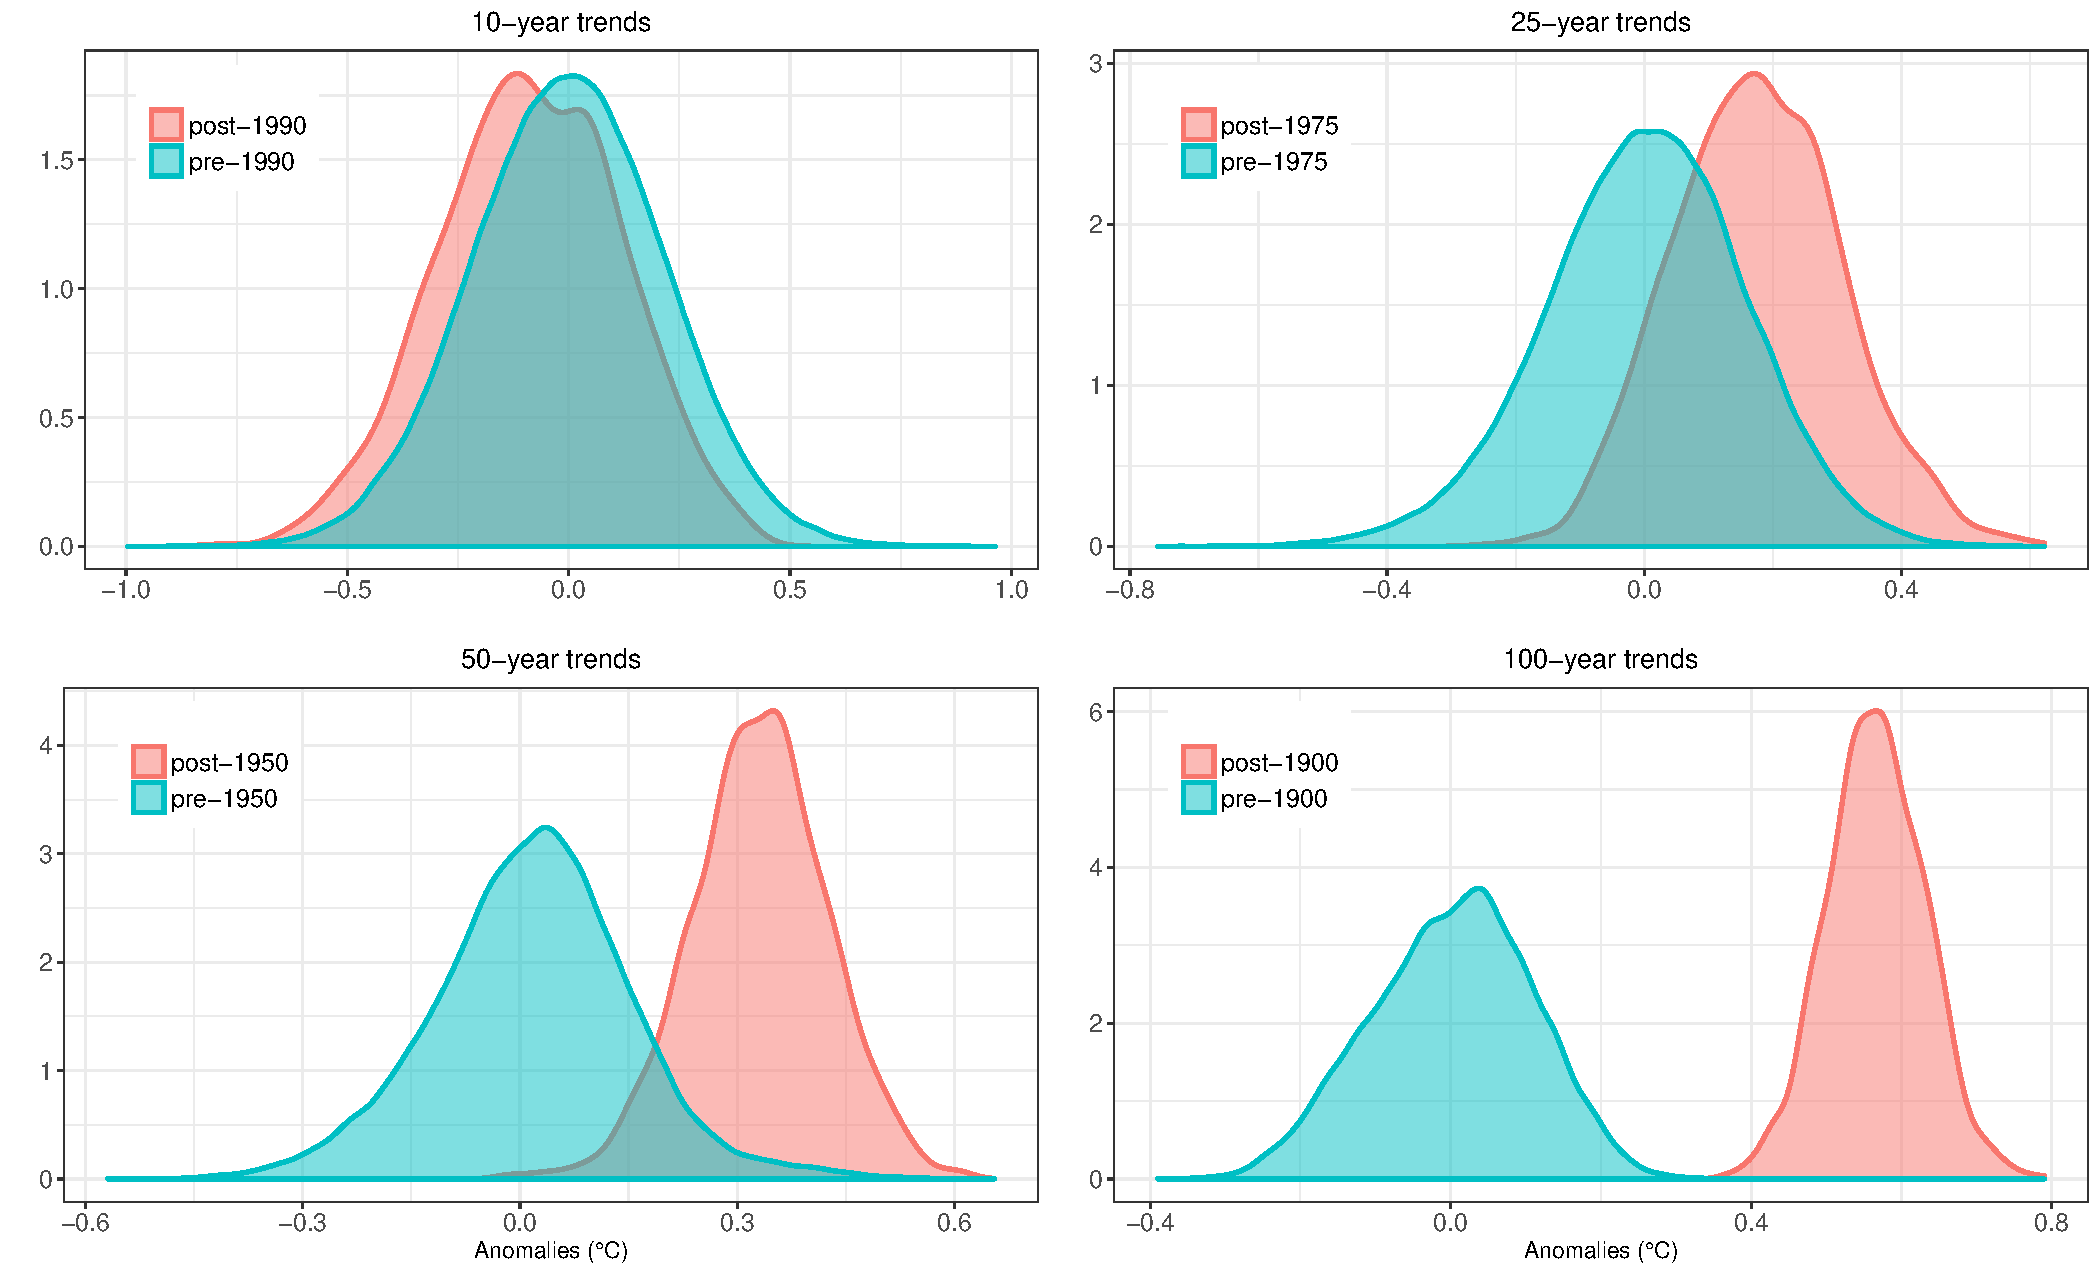
\includegraphics[scale=0.35]{compTrends}
  \caption{Comparison of the distribution of trends of reconstructed anomalies for different time horizons. Model sPCR-SSwF.}
  \label{fig:comptrends}
\end{figure}
\end{document}
